%% Преамбула TeX-файла

% 1. Стиль и язык
\documentclass[utf8x]{G7-32} % Стиль (по умолчанию будет 14pt) usepscyr

% Остальные стандартные настройки убраны в preamble.inc.tex.
\sloppy

% Настройки стиля ГОСТ 7-32
% Для начала определяем, хотим мы или нет, чтобы рисунки и таблицы нумеровались в пределах раздела, или нам нужна сквозная нумерация.
\EqInChapter % формулы будут нумероваться в пределах раздела
\TableInChapter % таблицы будут нумероваться в пределах раздела
\PicInChapter % рисунки будут нумероваться в пределах раздела

% Добавляем гипертекстовое оглавление в PDF
\usepackage[
bookmarks=true, colorlinks=true, unicode=true,
urlcolor=black,linkcolor=black, anchorcolor=black,
citecolor=black, menucolor=black, filecolor=black,
]{hyperref}

%\usepackage{pythonhighlight}


\makeatletter
\usepackage{color}
\definecolor{lightgray}{rgb}{0.95, 0.95, 0.95}
\definecolor{darkgray}{rgb}{0.4, 0.4, 0.4}
%\definecolor{purple}{rgb}{0.65, 0.12, 0.82}
\definecolor{editorGray}{rgb}{0.95, 0.95, 0.95}
\definecolor{editorOcher}{rgb}{1, 0.5, 0} % #FF7F00 -> rgb(239, 169, 0)
\definecolor{editorGreen}{rgb}{0, 0.5, 0} % #007C00 -> rgb(0, 124, 0)
\definecolor{orange}{rgb}{1,0.45,0.13}
\definecolor{olive}{rgb}{0.17,0.59,0.20}
\definecolor{brown}{rgb}{0.69,0.31,0.31}
\definecolor{purple}{rgb}{0.38,0.18,0.81}
\definecolor{lightblue}{rgb}{0.1,0.57,0.7}
\definecolor{lightred}{rgb}{1,0.4,0.5}
\usepackage{upquote}
\usepackage{listings}
\usepackage{lipsum}
\usepackage{markdown}

\lstdefinestyle{py} {%
language=python,
literate=%
*{0}{{{\color{lightred}0}}}1
{1}{{{\color{lightred}1}}}1
{2}{{{\color{lightred}2}}}1
{3}{{{\color{lightred}3}}}1
{4}{{{\color{lightred}4}}}1
{5}{{{\color{lightred}5}}}1
{6}{{{\color{lightred}6}}}1
{7}{{{\color{lightred}7}}}1
{8}{{{\color{lightred}8}}}1
{9}{{{\color{lightred}9}}}1,
basicstyle=\footnotesize\ttfamily, % Standardschrift
numbers=left,               % Ort der Zeilennummern
%numberstyle=\tiny,          % Stil der Zeilennummern
%stepnumber=2,               % Abstand zwischen den Zeilennummern
numbersep=5pt,              % Abstand der Nummern zum Text
tabsize=4,                  % Groesse von Tabs
extendedchars=true,         %
breaklines=true,            % Zeilen werden Umgebrochen
keywordstyle=\color{purple}\bfseries,
frame=b,
commentstyle=\color{brown}\itshape,
stringstyle=\color{editorGreen}\ttfamily, % Farbe der String
showspaces=false,           % Leerzeichen anzeigen ?
showtabs=false,             % Tabs anzeigen ?
xleftmargin=17pt,
framexleftmargin=17pt,
framexrightmargin=5pt,
framexbottommargin=4pt,
%backgroundcolor=\color{lightgray},
showstringspaces=false,      % Leerzeichen in Strings anzeigen ?
}%

\lstdefinestyle{htmlcssjs} {%
  % General design
%  backgroundcolor=\color{editorGray},
  basicstyle={\footnotesize\ttfamily},
  frame=b,
  % line-numbers
  xleftmargin={0.75cm},
  numbers=left,
  stepnumber=1,
  firstnumber=1,
  numberfirstline=true,
  % Code design
  identifierstyle=\color{black},
  keywordstyle=\color{blue}\bfseries,
  ndkeywordstyle=\color{editorGreen}\bfseries,
  stringstyle=\color{editorOcher}\ttfamily,
  commentstyle=\color{brown}\ttfamily,
  % Code
  language=HTML5,
  alsolanguage=JavaScript,
  alsodigit={.:;},
  tabsize=2,
  showtabs=false,
  showspaces=false,
  showstringspaces=false,
  extendedchars=true,
  breaklines=true,
  % German umlauts
  literate=%
  {Ö}{{\"O}}1
  {Ä}{{\"A}}1
  {Ü}{{\"U}}1
  {ß}{{\ss}}1
  {ü}{{\"u}}1
  {ä}{{\"a}}1
  {ö}{{\"o}}1
}

% Изменение начертания шрифта --- после чего выглядит таймсоподобно.
% apt-get install scalable-cyrfonts-tex

\IfFileExists{cyrtimes.sty}
    {
        \usepackage{cyrtimespatched}
    }
    {
        % А если Times нету, то будет CM...
    }

\usepackage{graphicx}   % Пакет для включения рисунков
\DeclareGraphicsExtensions{.jpg,.pdf,.png}
% С такими оно полями оно работает по-умолчанию:
% \RequirePackage[left=20mm,right=10mm,top=20mm,bottom=20mm,headsep=0pt]{geometry}
% Если вас тошнит от поля в 10мм --- увеличивайте до 20-ти, ну и про переплёт не забывайте:
\geometry{right=20mm}
\geometry{left=30mm}

\usepackage{subfig}
\renewcommand\thesubfigure{\asbuk{subfigure}}

% Произвольная нумерация списков.
\usepackage{enumerate}

\usepackage{amsmath}

\usepackage[normalem]{ulem}

\onehalfspacing

\setcounter{tocdepth}{2} %Подробность оглавления
%4 это chapter, section, subsection, subsubsection и paragraph
%3 это chapter, section, subsection и subsubsection
%2 это chapter, section, и subsection
%1 это chapter и section
%0 это chapter.


\begin{document}

\begin{center}
    Федеральное государственное автономное образовательное учреждение высшего образования\\
    «Московский физико-технический институт \pt(государственный~университет)»\\

    Физтех-школа радиотехники и компьютерных технологий\\
    Кафедра перспективных вычислительных технологий\\
\end{center}

\noindent
\textbf{Направление подготовки:} 03.04.01 Прикладные математика и физика\\
\textbf{Направленность (профиль) подготовки:} Электронные  вычислительные машины. Вычислительная техника\\

\begin{center}

    \textbf{УСТОЧЙИВОЕ ПРЕДСТАВЛЕНИЕ АУДИОСИГНАЛОВ ДЛЯ ЗАДАЧ СИНТЕЗА РЕЧИ}\\
    (магистерская диссертация)\\[15mm]

\end{center}


\hfill\begin{tabular}{@{}p{.5\linewidth}@{}}

    \textbf{Студент:}\\
    Панюков Александр Дмитриевич, группа М01-306б\\
    \uline{\hfill}\\
    \begin{center}\textit{(подпись студента)}\end{center}\\

    \textbf{Научный руководитель:}\\
    Горбацевич Владимир Сергеевич,\\
    к.ф.-м.н\\
    \uline{\hfill}\\
    \begin{center}\textit{(подпись научного руководителя)}\end{center}\\

\end{tabular}


\vfill

\begin{center}
    Москва, 2025
\end{center}

\thispagestyle{empty}

\chapter*{\centering Аннотация}

% - аннотация (не более 1500 знаков)
%   - цели и задачи работы
%   - полученные результаты
%   - рекомендации, предложенные на основании данной работы


\frontmatter % выключает нумерацию ВСЕГО; здесь начинаются ненумерованные главы: реферат, введение, глоссарий, сокращения и прочее.
\setcounter{page}{3}

\tableofcontents

% \chapter{\centering Обозначения и сокращения}

% - обозначения и сокращения

\Introduction

В наше время активно развиваются технологии искусственного интеллекта, помогая человеку взаимодействовать с цифровым миром в понятной и удобной ему форме. 
К таким технологиям можно отнести голосовых ассистентов, переводчиков на разные языки, ИИ-агентов, помогающих человеку выполнять различные задачи.
Также искусственный интеллект открывает человеку новые возможности для творчества с помощью технологий генерации контента, такого как изображения, музыка, пение, речь.

Одной из важных составляющих упомянутых технологий является синтез речи. 
Несколько десятилетий назад возможность озвучить текст голосом, чтобы человек мог услышать и воспринять информацию, уже была прорывом. 
Причем качество сгенерированного звука заметно отличалось от звучания естесовенной речи, иногда даже резало слух, создавая эффект зловещей долины, или просто утомляя пользователя.
Также низкое качество синтезированной речи делает затруднительным ее применение в творческих сферах, таких как музыка, фильмы и игры.

В настоящее время технологии синтеза речи сильно продвинулись. Голосовые ассистенты стали умнее и их речь стала более естственной. 
Появились нейросети, способные генерировать песни по заданному тексту или мотиву (Suno \cite{SunoAI_Bark_2023}, Riffusion \cite{Riffusion}). 
Но следы того, что музыка или речь создана роботом, все еще сохраняются.
Кроме того, использование моделей ИИ для генерации звука требует использования вычислительной мощности, которая может быть недоступна некоторым мобильным устройствам.
Также существуют проблемы с вычислительной сложностью систем генерации речи в реальном времени (синхронный перевод, замена голоса). 
Они могут быть ограничены в вычислительной мощности, особенно если рассчитанны на широкую аудиторию пользователей с их устройствами.
Поэтому на данном этапе развития продолжается борьба за качество и скорость синтеза речи.

Задачи анализа и синтеза речи включают в себя кодирование/декодирование звукового сигнала в признаковое представление, более удобное для нейросети.
Этот процесс может происходить по-разному в зависимости от архитектуры нейросети и может быть источником ошибок и артефактов, либо быть вычислительно сложным.
В данной работе предлагается алгоритм кодирования звуковых данных (вокодер), который 
\begin{itemize}
    \item восстанавливает звук без потерь, 
    \item является вычислительно эффективным, по сравнению с нейросетевыми вокодерами,
    \item эффективен с точки зрения плотности полезной информации (использует Mel-шкалу частот \cite{MelScale}),
    \item устойчив к искажениям, порождаемым нейросетями, а также к некоторым полезным трансформациям
\end{itemize}
Эти свойства позволяют повысить соотношение качество/сложность в современных решениях синтеза речи.

Целью данной работы является разработка и теоретическое обоснование алгоритмического вокодера для задач синтеза речи, который будет обеспечивать высокое качество генерации звука в сочетании с нейросетями, при этом являясь вычислительно быстрым.


\mainmatter

\chapter{Обзор существующих подходов и теоретическая справка}
\label{cha:ch_1}


\section{Архитектуры нейронных сетей для синтеза речи}
Современные решения для преобразования текста в речь в основном устроены следующим образом: (cм. Рисунок \ref{fig:tts_pipeline})

\begin{enumerate}
    \item В начале текст токенизируется - преобразуется из строкового формата в последовательность лексем - токенов
    \item токенизированный текст преобразуется с помощью нейросети-энкодера во внутреннее признаковое представление
    \item используя текстовые признаки, нейросеть генерирует признаковое представление звука или спектрограмму. Этот модуль может быть многоуровненвым и сложным в зависимости от архитектуры.
    \item признакове представление звука декодируется в звуковой сигнал.
\end{enumerate}

\begin{figure}
  \centering
  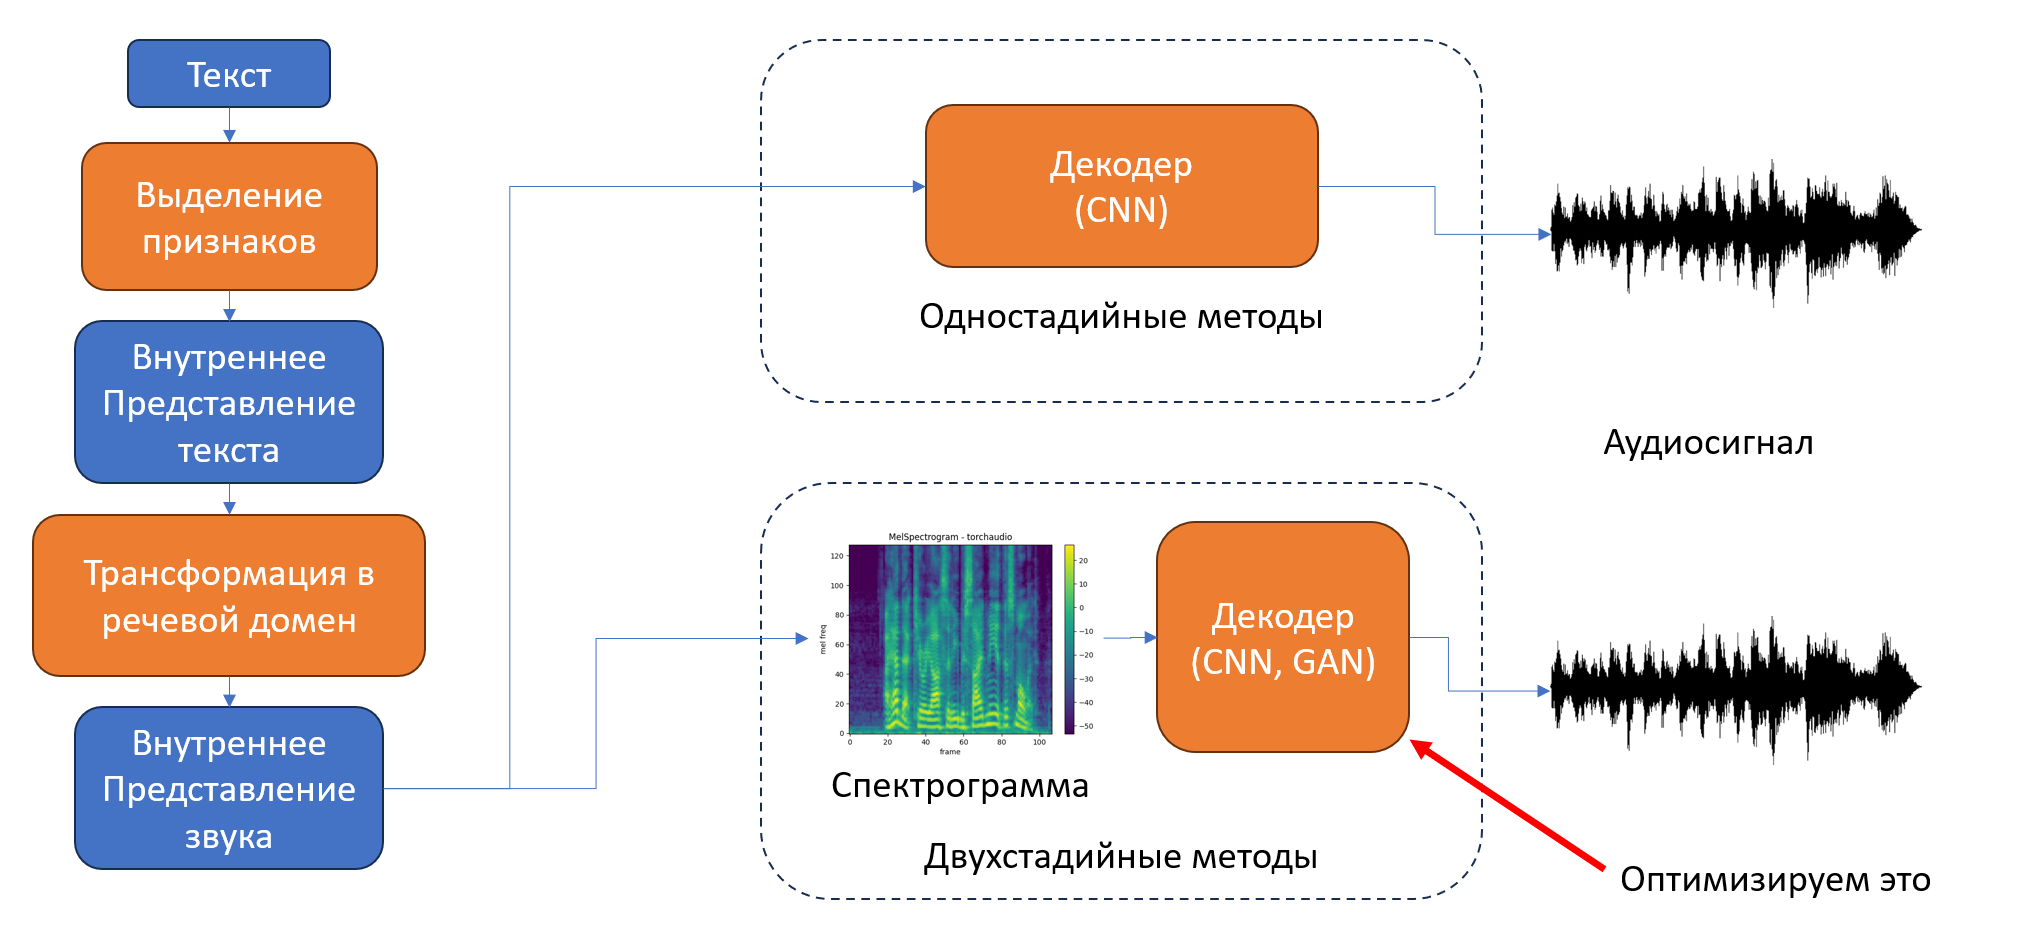
\includegraphics[width=16cm]{figures/tts_pipeline}
  \caption{Преобразование текста в речь}
  \label{fig:tts_pipeline}
\end{figure}

Также помимо задачи преобразования текста в речь, существуют задачи замены голоса, генерации музыки, перевода с сохранением голоса и прочие.
Их пайплайн устроен похожим образом, но какие-то части могут отличаться. 
Отметим, что в любой из перечисленных задач неотъемлемой частью пайплайна является этап декодирования звука из признакового представления в аудиосигнал.




\subsection{Понятие спектрограммы}
Прежде чем продолжить рассмотрение современных подходов для синтеза речи, раскроем понятие спектрограммы.

\textbf{Спектрограмма} - это двумерный массив данных, представляющий из себя разложение сигнала по спектру, изменяющееся во времени.
Такое разложение можно получить например с помощью оконного преобразования Фурье или вейвлет-преобразования. 
По горизонитальной оси отложено время в линейной шкале. По вертикальной оси отложены частоты, в некоторой шкале, не обязательно линейной.
На практике используются линейная, логарифмическая и мел-шкала.
\begin{itemize}
  \item Линейная шкала используется обычно в обратимых алгоритмоах или как разложение для передачи многоканальной информации в одном сигнале.
  \item Логарифмическая шкала используется в музкальных приложениях и редакторах.
  \item мел-шкала используется для анализа голоса. Она построена на исследованиях чувствительности человеческого слуха к изменению частоты.
\end{itemize}

На рисунке \ref{fig:log_spec} изображен пример спектрограммы в логарифмической шкале, а на рисунке \ref{fig:mel_spec} - в мел-шкале.
\begin{figure}
  \centering
  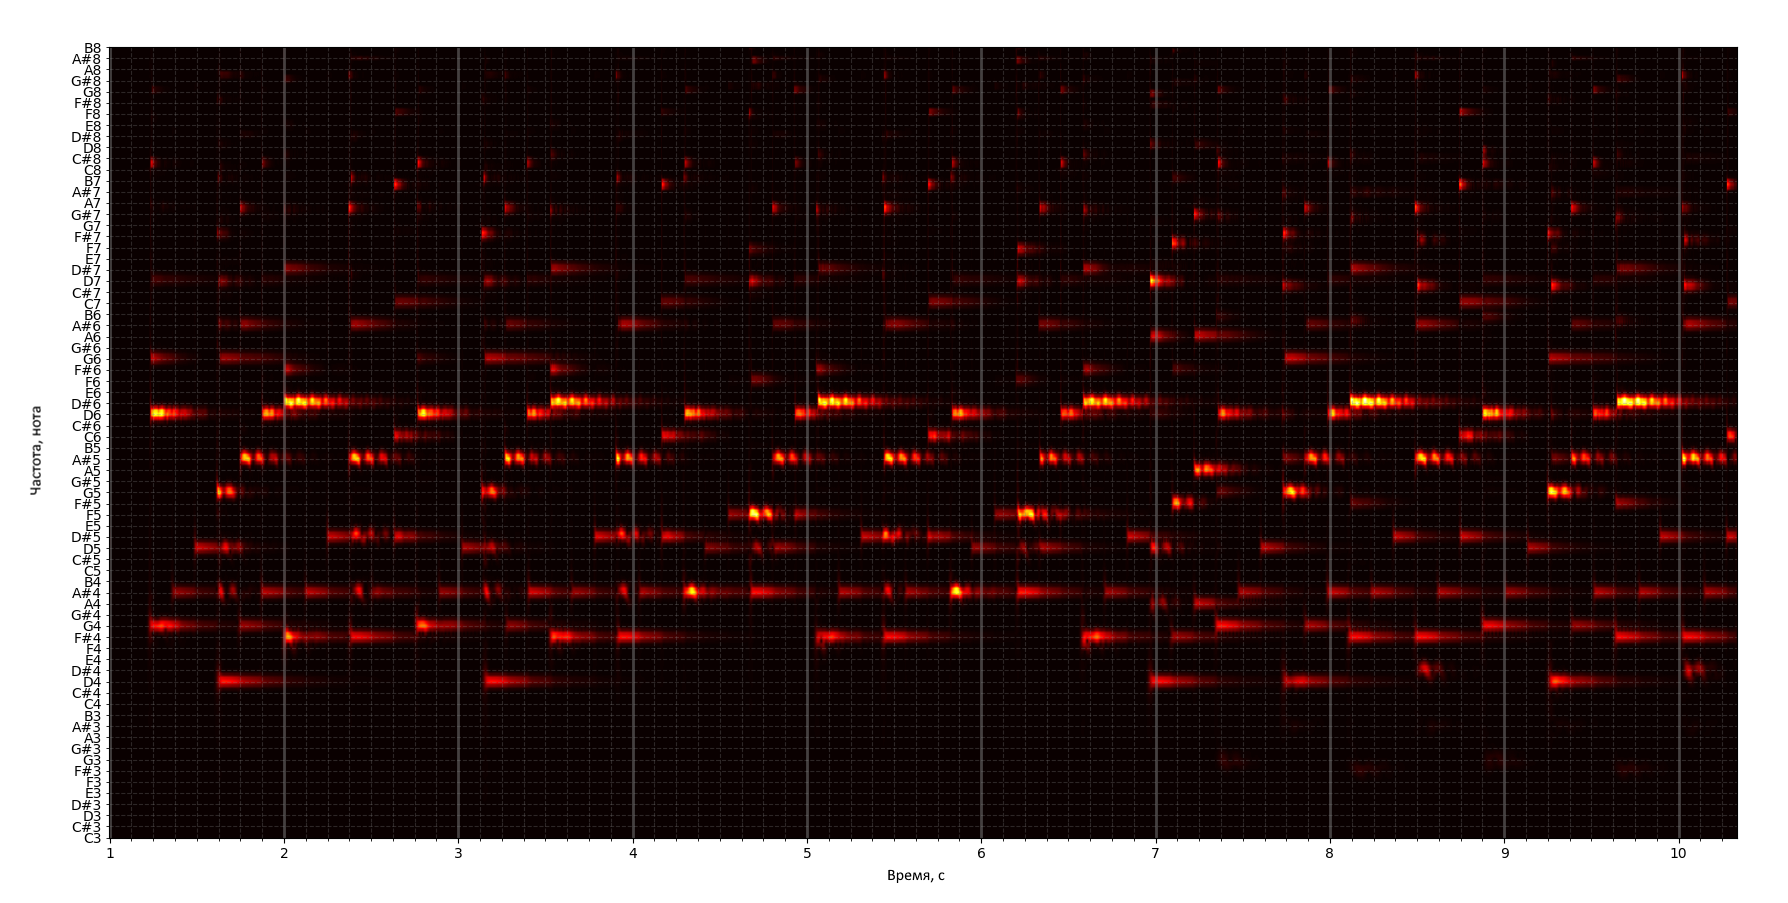
\includegraphics[width=16cm]{figures/log_spec}
  \caption{Спектрограмма записи игры на металлофоне в логарифмической шкале частот с указанием нот}
  \label{fig:log_spec}
\end{figure}

\begin{figure}
  \centering
  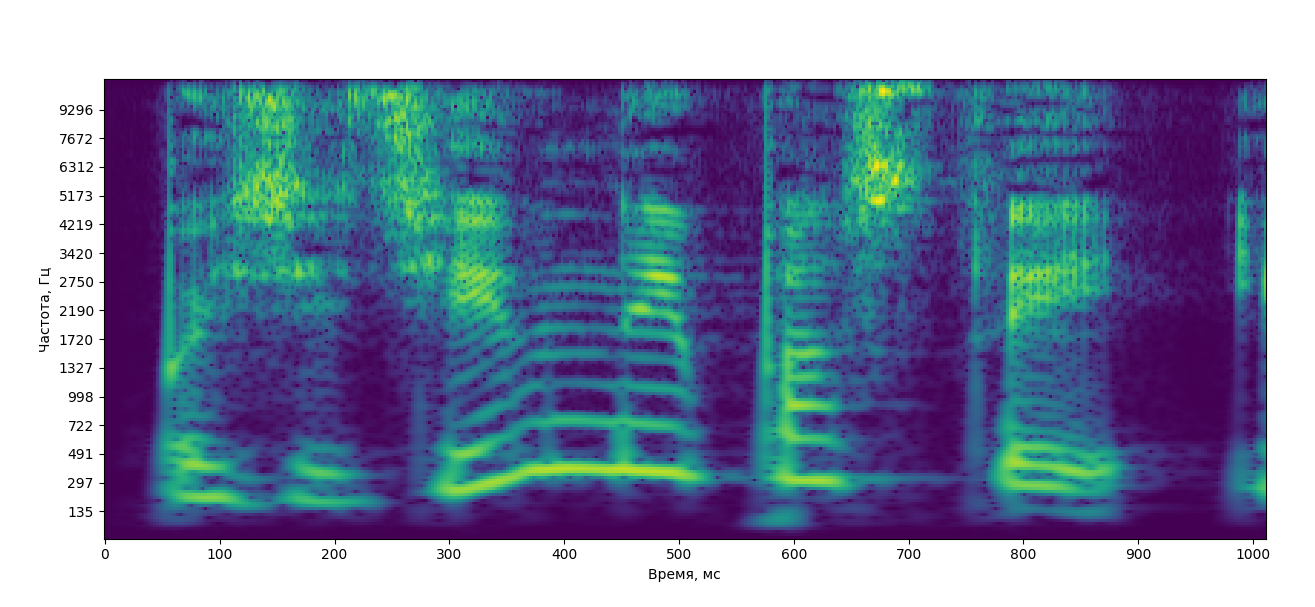
\includegraphics[width=16cm]{figures/mel_spec}
  \caption{Спектрограмма записи голоса в мел-шкале}
  \label{fig:mel_spec}
\end{figure}




\subsection{Классификация моделей}
Рассмотрим основные подходы, использующиеся в современных решениях синтеза речи и их классификацию.


\subsubsection{По формату промежуточного представления}
По формату промежуточного представления методы делятся на несколько типов:

\textbf{Генераторы спектрограмм} подразумевают генерацию спектрограммы с последующим преобразованием спектрограммы в звуковой сигнал. Примеры таких моделей:
\begin{itemize}
  \item Tacotron 2 (Google, 2017) \cite{Tacotron2} - классическая модель, использующая последовательное преобразование текста в мел-спектрограмму, с последующим применением вокодера для декодирвоания звука.
  \item FastSpeech 2 (Microsoft, 2019–2020) \cite{FastSpeech2} - Ускоренные и более стабильные версии Tacotron.
  \item Riffusion (2022) \cite{Riffusion} - Диффузионная модель, генерирующая песни и инструментальную музыку в виде спектрограмм с последующим декодированием в звук.
  \item TalkNet (2020, NVIDIA) \cite{TalkNet} - Полносверточная text-to-speech модель
\end{itemize}

\textbf{Генераторы в латентное представление} с последующим декодированием в звук с помощью нейронного декодера подразумевают 
генерацию латентного признакого представления, чем-то отдаленно схожего со спектрограммой, но сформированного отдельно обученным автоэнкодером.

\begin{itemize} 
  \item NaturalSpeech 2 (Microsoft, 2023) \cite{NaturalSpeech2} - Современная модель на основе латентных диффузий для синтеза речи и пения
  \item Kokoro-TTS (2025) \cite{kokoro}- это современная, компактная и высокоэффективная модель синтеза речи, разработанная для генерации естественного звучания при минимальных вычислительных затратах
\end{itemize}

\textbf{Генераторы токенов для нейронного кодека} схожи по принципу работы с генеративными трансформерами - основная генеративная модель создает последовательность токенов, 
которая потом преобразуется в звук с помощью нейросетевого кодека.

Пример такого кодека - EnCodec (Meta AI, 2022) \cite{encodec}. Он предназначен для сжатия и восстановления аудиосигналов, кодирует звук в дискретное латентное пространство (токены).

\begin{itemize} 
  \item Bark (Suno AI) \cite{SunoAI_Bark_2023} - Трансформерная генеративная модель, синтезирующая музыку и песни по заданному тексту и указаниям.
  \item Voicebox (2023, Meta AI) \cite{le2023voicebox} - Модель, способная генерировать, изменять и редактировать речь в различных стилях.
  \item VALL-E (Microsoft, 2023) \cite{Valle} - генерация речи с имитацией голоса на основе аудиопримера, на базе условной языковой модели.
\end{itemize}

\textbf{Одностадийные end-to-end аудиогенераторы} синтезируют звук напрямую, минуя стадию спектрограммы или отдельного декодера из латентного пространства.

\begin{itemize} 
  \item WaveNet (DeepMind, 2016) \cite{WaveNet} - Первая модель, которая напрямую генерировала звук по аудиосэмплам. Медленная, так как работает сэмпл за сэмплом (для аудио с частотой дискретизации 24 000 Гц — таких генераций должно быть 24 тысячи в секунду).
  \item DiffWave (Google, 2020) \cite{DiffWave} - Диффузионная модель, которая работает не со спектрограммой, а напрямую с аудиоволной. Высокое качество, но относительно медленная генерация.
\end{itemize}



\subsubsection{По принципу генерации промежуточного представления}
Если рассматривать принцип генерации промежуточного представления, то наиболее успешными являются трансформерные и диффузионные модели.
Также можно выделить полносверточные модели для обработки/восстановления звука, хотя существуют и полносверточные text-to-speech модели.


\textbf{Трансформерные генераторы} используют в качестве \textit{генератора} звукового представления GPT-подобный трансформер.
\begin{itemize}
  \item FastSpeech 2 (Microsoft, 2019–2020) \cite{FastSpeech2}
  \item Voicebox (2023, Meta AI) \cite{le2023voicebox}
  \item Bark (Suno AI) \cite{SunoAI_Bark_2023}
  \item Kokoro-TTS (2025) \cite{kokoro} - Поддерживает трансформеры в генераторе (настраиваемо)
  \item VALL-E (Microsoft, 2023) \cite{Valle} - генерация речи с имитацией голоса на основе аудиопримера, на базе условной языковой модели.
\end{itemize}

\textbf{Диффузионные генераторы} генерируют представление звука с помощью процесса обратной диффузии.
\begin{itemize}
  \item DiffWave (Google, 2020) \cite{DiffWave}
  \item NaturalSpeech 2 (Microsoft, 2023) \cite{NaturalSpeech2}
  \item Riffusion (2022) \cite{Riffusion}
\end{itemize}

\textbf{Полносверточные модели}
\begin{itemize} 
  \item TalkNet (2020, NVIDIA) \cite{TalkNet} - Полносверточная text-to-speech модель. В ней присутствуют отдельные полносверточные модели для предсказания длительности каждого текстового токена и модель для генерации спектрограмм. Очень быстрое обучение и синтез.
  \item Kokoro-TTS \cite{kokoro} в некоторых конфигурациях также может использовать полносверточный генератор с предсказанием длительности токенов, вместо трансформера.
  \item VoiceFixer (2022) \cite{VoiceFixer} - Восстановление повреждённой речи (например, из телефона, старых записей)
\end{itemize}


\section{Cуществующие вокодеры}
Среди существующих вокодеров, применяемых в современных системах синтеза речи, можно выделить следующие группы.

\textbf{Нейросетевые декодеры из спектрограммы} - HiFi-Gan \cite{hifigan}, WaveGlow \cite{WaveGlow} - восстанавливают звук из mel-спектрограммы
при помощи сверточных генеративных сетей. Информация в mel-спектрограмме может быть не полной или слегка искаженной, 
нейросеть все равно будет способна восстанавливать звук хорошего качества.

\textbf{Специализированные автоэнкодеры} - Сверточные сети, обученные под конкретную модель генератора. Так же способны генерировать звук хорошего качества, 
при этом часто работают быстрее, чем спектрограммные нейросетевые декодеры. Однако, под конкретную задачу и модель чаще всего требуется обучать отдельный 
автоэнкодер на большом объеме данных.

\textbf{Нейросетевые кодеки в дискретное латентное пространство} - EnCodec \cite{encodec} - кодирует звук в последовательность токенов. 
Может достигать хорошего качества в сочетании с трансформерами, и работает относительно быстро. Однако, в приложениях с большим разнообразием звуков и интонаций 
наблюдаются проблемы с качеством. А также этот кодек не работает с диффузионными и полносверточными генераторами.

\textbf{Алгоритмические декодеры из спектрограмм} - GriffinLim \cite{1164317} - Восстанавливает звук из спектрограммы (только магнитуды) в линейной шкале. 
Этот и другие алгоритмические декодеры могут восстанавливать звук точно без потерь. Но к сожалению при наложении небольших искажений,
пристуствующих в спектрограммах, сгенерированных нейросетью, появляются сильно заметные нежелательные артефакты (металлический звук, эхо), 
что делает такие декодеры неприменимыми в современных решениях. С другой стороны, такие декодеры заметно быстрее, чем нейросетевые, 
и могут быть использованы в приложениях для встраиваемых устройств с низкой вычислительной мощностью, когда можно пожертвовать качеством.


\subsection{Успехи и открытые проблемы}
Изучая успех упомянутых моделей среди сообщества и сравнивая качество синтезированного звука, можно сделать следующие выводы об успешности применения определенных технологий:

1. Существуют несколько технологий генерации звукового представления (диффузионные, трансформерные, полносверточные), способные синтезировать речь очень хорошего качества. Но такие технологии требуют больших вычислительных затрат. 
Есть оптимизированные решения, такие как Kokoro-TTS, достигающие высокого качества и высокой скорости работы за счет оптимизации архитектуры и размеров моделей, тщательной проработки и аккуратного обучения каждого компонента. 
Однако, у каждой технологии есть свои преимущества и недостатки, делающие ее более или менее пригодной для конкретной задачи.
Например: синтез музыки с множеством требований и указаний лучше всего удается диффузионным моделям. Полносверточные модели самые быстрые. 

2. Существует несколько типов вокодеров - использующие представление в виде спектрограммы, латентного представления, дискретного представления в виде токенов. Наилучшего качества в сочетании с нейросетями достигают нейросетевые вокодеры из латентного представления или спектрограммы. 
Алгоритмические вокодеры также существуют, но они неустойчивы к искажениям, которые неизбежно возникают при генерации представления с помощью нейросети, в результате чего появляются нежелательные артефакты.
Также для каждой технологии генерации подходит не любой тип промежуточного представления звука. Ниже рассмотрена совместимость технологий генерации с промежуточным представлением.

\begin{center}
\begin{tabular}{ c c c c }
                 & Спектрограмма & Латентное пр-е & Токены \\
    Диффузионные & +             & +              &        \\ 
  Трансформерные & +             & +              & +      \\  
 Полносверточные & +             & +              &     
\end{tabular}
\end{center}

Отсюда видно, что универсальными представлениями, работающими с любым типом генерации, являются спектрограмма и латентное векторное представление. 

3. Нейросетевой декодер из латентного пр-ва, обученный на одном наборе данных, 
может не подходить для применения на других данных (например на другом языке) или 
не подходить для конкретной задачи (учет интонации, акцента, персональности голоса говорящего).

4. Спектрограммные нейросетевые декодеры практически всегда требуют больших вычислительных затрат, чем из латентного пр-ва из-за избыточности информации. 
С другой стороны, в спектрограмме содержится достаточно информации для восстановления звука без потерь, 
и поэтому декодер из спектрограммы можно использовать для любой задачи, домена и технологии, и достигать наилучшего качества генерации.
Спектрограммное представление можно назвать \textit{универсальным} с точки зрения применимости технологии и задачи, но избыточным в плане вычислительных ресурсов 
(при использовании нейросетевого декодера).

5. Модели, генерирующие непосредственно звуковой сигнал, работают медленно и сложны в обучении. Практически всегда их можно разделить на две стадии - предобучение нейросетевого автоэнкодера в латентное пр-во и генерация на этом пр-ве.

6. Если бы существовал алгоритмический декодер спектрограммы, способный восстанавливать аудиосигнал с качеством, 
сопоставимым с современными нейросетевыми вокодерами, при этом устойчивый к искажениям во входных данных и обладающий более высокой скоростью работы на CPU, 
это могло бы упростить архитектуру TTS-систем, сократить вычислительные затраты и повысить доступность синтеза речи. 
Кроме того, использование стандартизированного формата спектрограмм позволило бы сосредоточить усилия на улучшении генератора, 
ускорить обучение и повысить воспроизводимость моделей.


\section{Спектральный анализ аудиосигналов}
В данном разделе рассмотрим теоретические основы алгоритмов построения спектрограмм и способы восстановления звукового сигнала из таких представлений.

Для начала рассмотрим \textbf{Оконное преобразование Фурье} или в англоязычной литературе Short-Time Fourier Transform (\textbf{STFT}) \cite{STFT}.

Оно представляет из себя двумерную функцию (от частоты и от времени), определяемую как преобразование Фурье от сигнала, умноженного на оконную функцию, сдвинутую во времени:

\begin{equation}
  \textbf{STFT}\{x(t)\} (\tau, \omega) = \int_{-\infty}^\infty x(t) w(t - \tau) e^{-i\omega t} dt
  \label{eq:stft_cont}
\end{equation}

Здесь \(w(t)\) - оконная функция. От ее выбора зависит разрешение спектрограммы по времени и по частоте. Иллюстрация работы STFT приведена на рисунке \ref{fig:mel_spec}.
В результате такого преобразования получается спектрограмма в линейной шкале, на которой можно увидеть, как разложение сигнала по частотам (спектр), изменяется во времени.

\begin{figure}
  \centering
  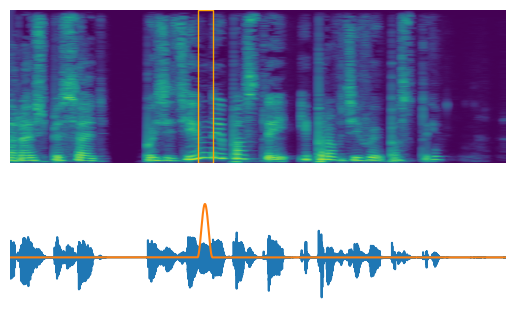
\includegraphics[width=16cm]{figures/stft}
  \caption{Оконное преобразование Фурье (STFT)}
  \label{fig:stft}
\end{figure}

На практике используется дискретное оконное преобразование Фурье.
\begin{equation}
  \textbf{STFT}\{x[n]\} (m, k) = \sum_{n=0}^{N-1} x[n] w[n - m] e^{-2\pi i  \frac{k n}{N}} = \textbf{DFT}\{x[m:m+N] * w[0:N]\}(k)
  \label{eq:stft}
\end{equation}
Алгоритм его построения обычно следующий - из сигнала \(x[n]\) вырезается отрезок длиной \(N\) отсчетов со сдвигом по времени \(m\) отсчетов. 
Результат ДПФ выделенной части сигнала, умноженной на окно, присоединяется к массиву. В результате получается массив \([M \times K]\), 
представляющий из себя спектрограмму, как на рисунке \ref{fig:stft}

\begin{wrapfigure}{r}{0.4\textwidth}
  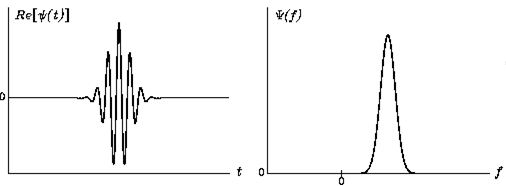
\includegraphics[width=0.9\linewidth]{figures/wavelet}
  \caption{Временное и спектральное представления вейвлета Морле \cite{MorleWavelet}}
  \label{fig:wavelet}
\end{wrapfigure}

Несложно показать, что преобразование является линейным, как и ДПФ.
Также можно представить каждый элемент $\textbf{STFT}\{x[n]\} (m, k)$ как свертку сигнала $x[n]$ с вейвлетом $w[n - m] e^{-2\pi i  \frac{k n}{N}}$.
И всю спектрограмму можно построить с помощью вейвлет-преобразования. Более того, для каждой частоты вейвлета можно выбирать свою ширину окна: 
$\psi_{k,m}(n) = w_k[n - m] e^{-2\pi i  \frac{k n}{N}}$. По такому принципу построено вейвлет-преобразование на основе вейвлета Морле \cite{MorleWavelet}, 
окном которого выбрана Гауссовская функция с шириной в несколько периодов соответствующей частоты. Это преобразование обратимо, так же как и STFT.

Рассмотрим влияние оконных функций на разрешение по времени и частоте. 
Оконная функция необходима для локализации события во временной области. 
Спектр оконной функции покажет, насколько хорошо событие локализовано в частотной области.
Кроме того, широкий спектр окна с паразитными "хвостами" создает связанность отдаленных частот. 
Небольшое искажение на одной частоте сильно влияет на другие частоты из-за таких эффектов, если не согласовано с этими частотами, 
чтобы в резульате интерференции получалось нужное значение. Примеры оконных функций и их спектров рассмотрены на рисунке \ref{fig:windows}

\begin{figure}[t]
  \centering
  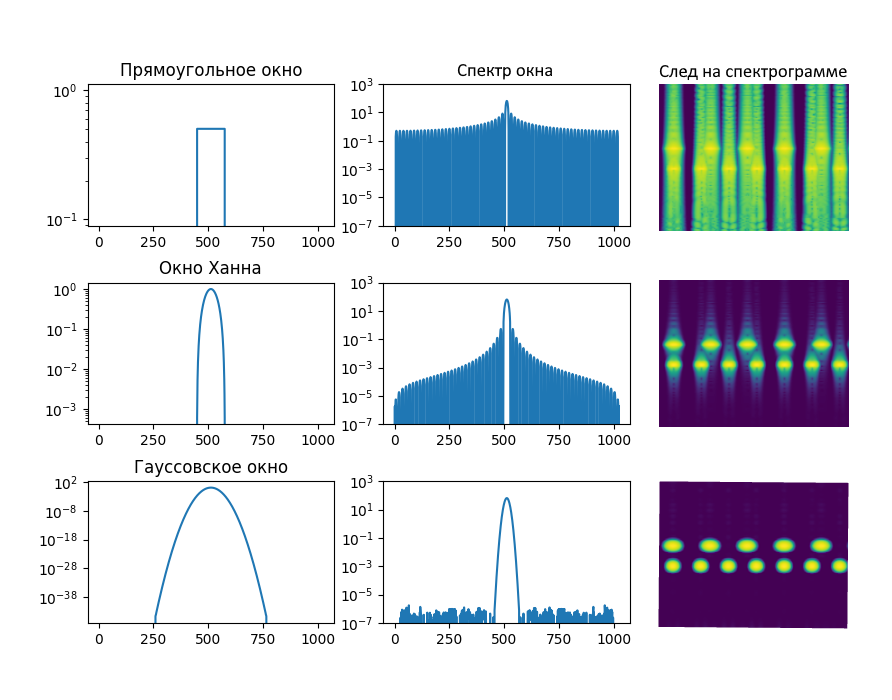
\includegraphics[width=16cm]{figures/windows}
  \caption{Сравнение оконных функций}
  \label{fig:windows}
\end{figure}

По отношению к оконным функциям, а также любым сигналам, над которыми производится спектральное преобразование, сущетвует принцип неопределенности, который гласит, что
для дифференцируемых вещественных сигналов 
$x(t)$ с энергией $E$, для которых интеграл 
$t_{0} = \int \limits _{-\infty }^{\infty }tx^{2}(t)dt$ сходится и $\lim _{t\to \pm \infty }tx^{2}(t)=0$, произведение эффективной длительности сигнала 
$\Delta t$ и эффективной ширины полосы частот сигнала $\Delta f$ ограничено снизу \cite{Umnyashkin}:
\begin{equation}
  \Delta t\Delta f\geq {\frac {E}{\pi }}
  \label{eq:uncertainity}
\end{equation}
Равенство $\Delta t\Delta f={\frac {E}{\pi }}$ достигается только в случае гауссова импульса $x(t)=Ce^{-kt^{2}}$, где 
$k$ и $C$ - некоторые константы ($k>0$). \cite{Umnyashkin}

Это отношение применимо и к оконным функциям, и к вейвлетам, которые являются базисом для разложения. 
В контексте спектрограммы принцип неопределенности проявится в размытии образа сигналов на соседние частоты и времена с шириной $\Delta t$ и $\Delta f$.
Иллюстрацию этого явления можно увидеть на рисунке \ref{fig:windows}

Рассмотрим подробно окно в виде гауссовской функции. Его спектр представлен также гауссовской функцией. Хоть она и является инфинитной (не равна нулю на всей шкале времени),
но приближается к нулю с экспоненциальной скоростью. Хотя финитный сигнал не может иметь финитный спектр, 
такое окно вполне удовлетворяет практическим сценариям применения и имеет понятный физичиский смысл - локализация события имеет нормальное распределение.
Как было показано, Гауссовское окно обладает наилучшими характеристиками для локализации событий одновременно в частотной и во временной области.
Это окно используется в преобразовании Габора \cite{Gabor} (STFT с гауссовским окном) и вейвлетах Морле \cite{MorleWavelet}.

Кроме того, при использовании гауссовского окна в прямом и обратном преобразовании, искажения, наложеннные на спектрограмму в одном месте, наложат сильно ограниченные по времени и частоте изменения в сигнал 
(преобразование является линейным, поэтому его след в частотно-временном представлении будет результатом свертки окна с искажением), 
что придает обратному преобразованию большую устойчивость к искажениям, чем при использовании любого другого окна. 
Поэтому в данной работе предлагается использование именно гауссовского окна.

\subsection{Естественная для человеческого слуха шкала амплитуд и частот}
Используемые в задачах синтеза речи способы представления аудиосигнала, такие как мел-спектрограмма, опираются на исследования восприятия человеком звука, 
его чувствительности к громкости и тональности звуков. 

Для задач генерации звука с помощью нейросетей важно построить шкалу, 
на которой изменение частоты $\Delta f$ или амплитуды $\Delta a$ будет одинаково ощущаться человеком при любом абсолютном значении частоты или амплитуды.
Это связано с тем, что при обучении нейросети возникают погрешности, ограниченные снизу в зависимости от learning rate. 
Обучение нейросети представляет собой минимизацию ошибки. 
И если лосс-функция одинаково чувствительна к ошибке на всем диапазоне значений, то обучение идет более равномерно и стабильно, и приводит к лучшим результатам,
чем когда чувстительность лосс-функции сильно различается в зависимости от абсолютного значения.
При правильной постановке задачи обучения чувствительность лосс-функции к ошибке нейросети должна быть пропроциональна чувствительности человечекого слуха к этой ошибке. 
Поэтому, если в выходном представлении частоты и амплитуды будут расположены на шкале, на которой изменения в любом диапазоне ощущаются человеком одинаково, 
нейросеть сможет достичь лучшего качества синтезируемого звука.

Естественной для человеческого восприятия \textbf{шкалой громкости} звука является логарифмическая шкала или \textbf{децибелы}.
Еще в 19 веке было установлено, что характер отображения в органах чувств человека и животных изменений течения многих физических и 
биологических процессов пропорционален логарифму интенсивности раздражителя (эмипрический Закон Вебера — Фехнера).
Эта особенность делает применение логарифмических шкал, логарифмических величин и их единиц вполне естественным.
Многочисленные исследования показывают, что это относится и к восприятию громкости звука.

Теперь разберемся, что же означает громкость звука в децибелах. 
Если громкость звука (субъективно определяемая его интенсивностью) возросла на 10 дБ, то это значит, что интенсивность звука возросла в 10 раз.
Это можно выразить формулой:
\begin{equation}
  dB(I) = 10 * lg(\frac{I}{I_0})
\end{equation}
Отметим, что коэффициент 10 справедлив для энергетических величин. 
Если измеряется отношение силовых величин (амплитуда, звуковое давление), то интенсивность (энергетическая величина) пропорциональна их квадрату. 
Поэтому перед логарифмом нужно использовать коэффициент 20, чтобы получить такое же изменение, как и при логарифмировании энергетической величины.

Использование децибелов при указании громкости звука обусловлено человеческой способностью воспринимать звук в очень большом диапазоне изменений его интенсивности. 
Применение линейной шкалы оказывается практически неудобным. Кроме того, на основании закона Вебера — Фехнера, 
ощущение громкости звука пропорционально логарифму его интенсивности. Отсюда удобство логарифмической шкалы. 
Диапазон величин звукового давления от минимального порога слышимости звука человеком (20 мкПа) до максимального, 
вызывающего болевые ощущения, составляет примерно 120 дБ. 
Например, утверждение «громкость звука составляет 30 дБ» означает, что интенсивность звука в 1000 раз превышает порог слышимости звука человеком.
Для выражения громкости звука также используют единицы фон и сон, учитывающие частотную и субъективную восприимчивость звука человеком.

Стоит также уделить внимание наличию порога слышимости. Человек не может различать уровни громкости вблизи порога слышимости так же хорошо, 
как в привычном диапазоне. А если громкости двух звуков ниже этого порога, то в нужной нам естественной шкале они должны быть практически равны нулю.
Этого можно добиться, если в стандартную формулу децибела добавить слагаемое $1 +$ под логарифмом. 
В результате получим такую формулу перевода шкалы громкости для спектрограммы из интенсивности в децибелы.
\begin{equation}
  I_{db}[m, k] = 10 lg(1 + \frac{I[m, k]}{I_0}),
\end{equation}
где $I_0$ - интенсивность порога слышимости, определяется эмпирически. Интенсивность звука на спектрограмме $I[m,k]$ получается как 
квадрат модуля спектральной компоненты $\mathrm{spec}[m,k]$, поскольку спектр получен с помощью линейного преобразования от сигнала 
$x(t)$ - звукового давления микрофона от времени.

Стоит также осветить вопрос зависимости энергии звуковой волны от частоты. Поскольку в колебаниях и волнах энергия перетекает между потенциальной и кинетической,
полная энергия колебаний равна либо максимальной потенциальной, либо максимальной кинетической. 
Максимальная кинетическая энергия пропорциональна квадрату амплитуды скорости: $E \sim \dot{x}_0^2$. 
В синусоидальных колебаниях и волнах амплитуда скорости на заданной частоте пропорциональна амплитуде смещения, 
умноженной на частоту: $\dot{x}_0 = x_0 \cdot \omega = x_0 \cdot 2\pi f$. 
Отсюда, энергия колебаний $E \sim (x_0 \cdot f)^2$.

Если в аудиозаписи человеческого разговора посчитать для каждой частоты среднюю амплитуду смещения и среднюю амплитуду скорости (Рисунок \ref{fig:spectrum_mean}), 
можно увидеть, что амплитуда скорости распределена почти равномерно по частотам. Это означает, что человек при разговоре производит звук, 
энергия которого распределена по частотам почти равномерно. Поэтому следует ожидать, 
что и чувствительность слуха к изменению энергии (а значит и апмлитуды скорости) будет почти одинакова на разных частотах.

\begin{figure}
  \centering
  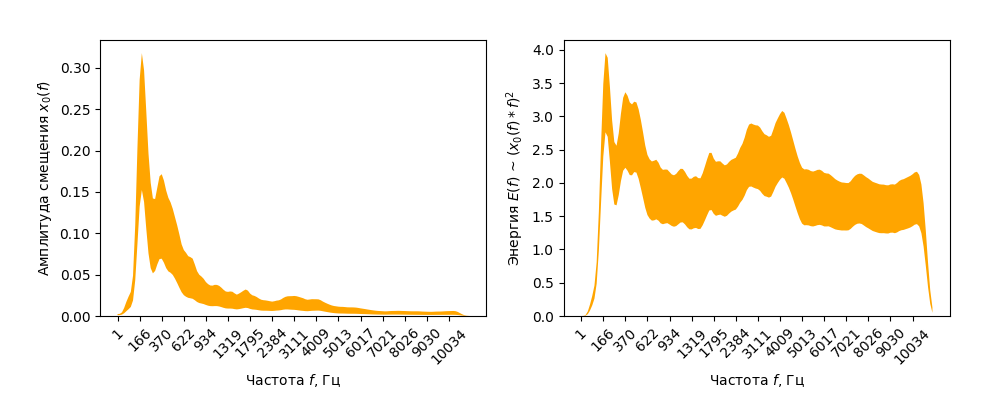
\includegraphics[width=0.9\linewidth]{figures/spectrum_mean}
  \caption{Средние амплитуды смещения и скорости на разных частотах в аудиосигнале}
  \label{fig:spectrum_mean}
\end{figure}


Теперь рассмотрим используемые в технике и акустике \textbf{шкалы частот}:

\textbf{Линейная} шкала используется в обратимых алгоритмах разложения сигнала, а также в системах передачи многоканальных данных по радиосвязи или в одном сигнале.
  
\textbf{Логарифмическая} шкала используется в музыке, в нотной системе (соседние ноты отличаются на $\sqrt[12]{2}$). 
Логарифмическое представление хорошо отражает чувствительность человеческого слуха к частоте, что и было положено в основу системы нот и подтверждается многими исследованиями.
Кроме того, у логарифмической шкалы есть полезное свойство - гармоники $f_n = n * f_0$ произвольной частоты $f_0$ будут расположены на 
фиксированном расстоянии от основной частоты на логарифмической шкале:
$log(f_n) - log(f_0) = log(n)$. В природе множество звуков издается стоячими волнами в резонаторах, которые излучают несколько гармоник, в том числе и человеческий голос.
И на логарифмической шкале спектрограммы двух звуков, созданных таким резонатором (гитара, флейта, голос), с разными опорными частотами, 
будут сдвинуты по шкале частот с сохранением расстояний между гармониками (но амплитуды каждой гармоники могут измениться). 
К проблемам логарифмической шкалы можно отнести то, что у человека существует верхний и нижний порог чувствительности частоты, 
за которыми начинаются ультразвук и инфразвук, не слышимые человеком. 
Логарифмическая шкала не учитывает изменения в чувствительности вблизи порогов слышимости.

\textbf{Мел-шкала} \cite{MelScale} частот основана на исследованиях о чувствительности человеческого слуха к изменению частоты. Название связано со словом "мелодия".
Частота по этой шкале измеряется в мелах. Расстояние между соседними частотами в 1 мел означает, что они едва различимы человеком.
Эмпирическая формула (О'Шонесси, 1987 \cite{oshaughnessy1987speech}) для перевода из $f$-герц в $m$-мелы выглядит так:
\begin{equation}
  m = 2595 \log_{10}(1 + \frac{f}{700}) = 1127 \ln(1 + \frac{f}{700})
\end{equation}


Теперь рассмотрим вопрос выбора ширины окна в зависимости от частоты и шкалы частот. 
Каждый элемент спектрограммы соответствует координате на плоскости частота-время $(f, t)$. Все координаты вместе образуют некую сетку, 
заполняющую частотно-временное пространство сигнала. 
Каждый элемент получается путем свертки сигнала с вейвлетом частоты $f$, расположенным во времени вокрут точки $t$.  
Исходя из формы окна вейвлета и соотношения неопределенности \ref{eq:uncertainity} для преобразования Фурье, 
эта свертка с вейвлетом позоляет захватывать временную область сигнала шириной $\Delta t$ и частотную область сигнала шириной $\Delta f$, 
которые связаны между собой соотношением неопределенности $\Delta t \Delta f = const \geq {\frac {E}{\pi }}$. Значение константы зависит от формы окна.

В линейной шкале все базисные элементы расположены равноудаленно по времени и частоте. 
Поэтому в линейной шкале одинаковый размер окна для любой частоты позволяет захватывать всю частотную область.
Выбрав окно с шириной спектра $\Delta f = f_{max} / N$, и подобрав шаг
по времени $\leq \Delta t$, можно покрыть полностью всё частотно-временное пространство сигнала.

\begin{wrapfigure}{r}{0.3\textwidth}
  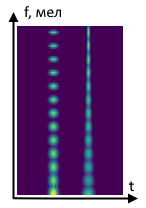
\includegraphics[width=0.9\linewidth]{figures/windows_mel}
  \caption{Одинаковая и переменная ширина окна в мел-шкале}
  \label{fig:windows_mel}
\end{wrapfigure}

Однако, в нелинейной шкале, такой как логарифмическая или мел-шкала, расстояния между соседними частотами различаются. 
Если в некоторой области частот ширина окна $\Delta f$ будет меньше разницы частот между соседними элементами спектрограммы (см. Рисунок \ref{fig:windows_mel}, слева),
то часть информации о сигнале будет утеряна, что сделает невозможным его точное восстановление.
Если же ширина окна $\Delta f$ будет больше разницы частот между соседними элементами спектрограммы, 
элементы будут накладываться друг на друга и перемешиваться,
что выражается в снижении эффективного разрешения спектрограммы по частоте.
При выборе для каждой опорной частоты $f$ своей спектральной ширины окна $\Delta f(f)$, пропорциональной расстоянию между соседними частотами на выбранной шкале, 
удается добиться оптимального разрешения по частоте и сохранить всю частотную информацию сигнала (см. Рисунок \ref{fig:windows_mel}, справа). 
Ширина окна по времени $\Delta t(f) = C / \Delta f(f)$ выбирается исходя из соотношения неопределенности.

С другой стороны, при таком выборе размеров окна, ширина $\Delta t(f)$ на высоких частотах может стать меньше шага сетки, что приведет к потере информации.
На низких частотах, где $\Delta t$ больше шага сетки, наоборот возникает наложение сигнала по времени, что приводит к избыточности информации в спектрограмме. 
Как мы увидим далее, такая избыточность не помешает восстановлению информации.


\subsection{Восстановление сигнала}
В данном разделе рассмотрим алгоритмы восстановления аудиосигнала из спектрограммы.

Если спектрограмма была построена с помощью оконного преобразования Фурье (STFT, Равенство \ref{eq:stft}), то для восстановления сигнала можно воспользоваться обратимостью ДПФ.
Для каждой координаты $m$ по времени можем получить фрагмент сигнала $x[n]$, умноженный на окно $w[n-m]$ в окрестности координаты $m$: 

\begin{equation}
  x_m[n] = \textbf{IDFT}\{spec[m](k)\}(n) = x[n]*w[n - m]
  \label{eq:idft}
\end{equation}

Останется правильным образом выполнить сшивку фрагментов сигнала, умноженных на окно, в единый сигнал.
Элемент сигнала $x[n]$ можно представить как взвешенную сумму

\begin{equation}
  x[n] = \frac{\sum_{m_i} x[n]*w[n-m_i]}{\sum_{m_i} w[n-m_i]}
\end{equation}

\begin{figure}
  \centering
  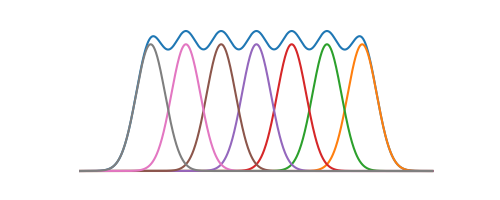
\includegraphics[width=0.8\linewidth]{figures/windows_sum}
  \caption{Окна с шагом как коэффициенты взвешенной суммы}
  \label{fig:windows_sum}
\end{figure}

Если посчитать заранее сумму всех окон $w_{sum}$ (\ref{eq:wsum}), то исходный сигнал $x[n]$ можно будет получить, 
просуммировав все сигналы $x_{m_i}[n]$ и разделив на $w_{sum}[n]$ (см. \ref{eq:istft_final})

\begin{equation}
  w_{sum}[n] = \sum_{m_i} w[n-m_i]
  \label{eq:wsum}
\end{equation}

\begin{equation}
  x[n] = \frac{\sum_{m_i} x_{m_i}[n]}{w_{sum}[n]} 
  \label{eq:istft_final}
\end{equation}


Для построения спектрограммы также можно использовать вейвлет-преобразование \cite{mallat2008wavelet}, 
которое строится на основе сверток вейвлет-функции $\psi(t)$ с сигналом $x(t)$.

Для осуществления и обратимости вейвлет-преобразования, вейвлет-функции должны удовлетворять следующим критериям:

Вейвлет $\psi(t)$ должен обладать конечной энергией: 
\begin{equation}
  E=\int \limits _{-\infty }^{\infty }{|\psi (t)|}^{2}\,dt<\infty
\end{equation}

Если ${\hat{\psi }}(f)$ - фурье-преобразование для вейвлета $\psi (t)$, то должно выполняться следующее условие:
\begin{equation}
  C_{\psi }=\int \limits _{0}^{\infty }{\frac {{|{\hat {\psi }}(f)|}^{2}}{f}}\,df<\infty
\end{equation}
Это условие называется условием допустимости (admissibility). Из него следует, что вейвлет должен иметь нулевое среднее 
(т.е. $\int_{-\infty}^{\infty}{\psi(t)}\,dt = 0$) и не должен содержать компоненту на нулевой частоте (${\hat{\psi }}(0) = 0$)

\textbf{Непрерывное вейвлет-преобразование} (CWT) \cite{mallat2008wavelet} определяется следующим образом:
\begin{equation}
  T(a,b)={\frac {1}{\sqrt {a}}}\int \limits _{-\infty }^{\infty }x(t)\psi ^{*}\left({\frac {t-b}{a}}\right)\,dt
\end{equation}
где ${\psi }^{*}$ означает комплексное сопряжение для $\psi$, параметр $b\in R$ соответствует временному сдвигу, и называется параметром положения, 
параметр $a>0$ задает масштабирование и называется параметром растяжения. 

Исходный сигнал может быть восстановлен по формуле обратного преобразования
\begin{equation}
  x(t)={\frac {1}{C_{\psi }}}\int \limits _{-\infty }^{\infty }\int \limits _{-\infty }^{\infty }T(a,b)\,{\psi }_{a,b}(t)\,da\,db}
\end{equation}

В дискретном случае, параметры масштабирования a и сдвига b представлены дискретными величинами: $a=a_{0}^{m},\quad b=nb_{0},\quad$где $m$ и $n$ — целые числа.

Тогда анализирующий вейвлет имеет следующий вид:
\begin{equation}
  \psi _{m,n}=a_{0}^{-m/2}\psi \left({\frac {t-nb_{0}}{a_{0}^{m}}}\right)
\end{equation}

В таком случае для непрерывного сигнала $x(t)$ дискретное вейвлет-преобразование и его обратное преобразование запишутся следующими формулами:
\begin{equation}
  {\displaystyle T_{m,n}=\int \limits _{-\infty }^{\infty }x(t)\,\psi _{m,n}^{*}(t)\,dt}
\end{equation}
Величины $T_{m,n}$ также известны как вейвлет-коэффициенты.
\begin{equation}
  x(t)=K_{\psi }\sum \limits _{m=-\infty }^{\infty }\sum \limits _{n=-\infty }^{\infty }T_{m,n}\psi _{m,n}(t)
\end{equation}
где $K_{\psi }$ — постоянная нормировки.

В данной работе применяется алгоритм, который во многом схож с дискретным вейвлет-преобразованием, но все же его точная формула отличается.


В результате как оконного преобразования Фурье, так и вейвлет-преобразования, получается набор комплексных коэффициентов $T_{m,n} \in \mathbb{C}$. 
Такое представление имеет амплитудную и фазовую составляющую (см. Рисунок \ref{fig:complex_spec}). 

\begin{figure}
  \centering
  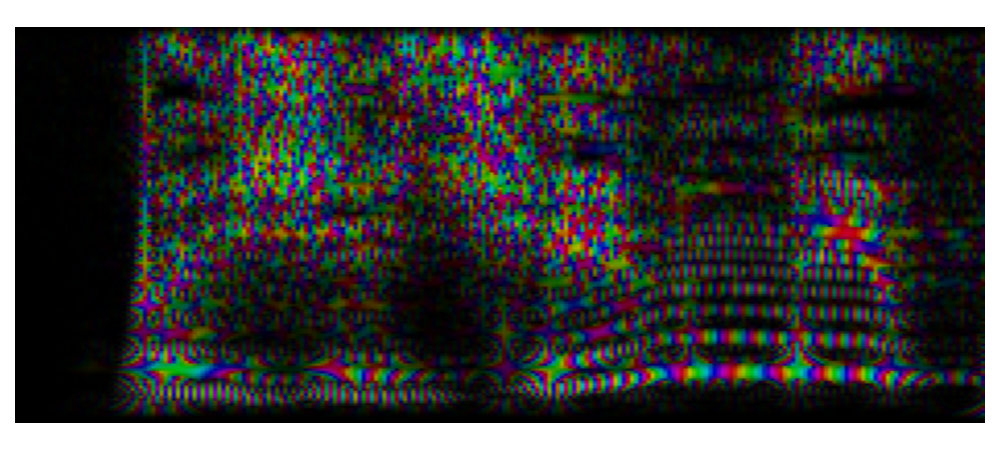
\includegraphics[width=0.9\linewidth]{figures/complex_spec}
  \caption{Комплексное представление спектрограммы}
  \label{fig:complex_spec}
\end{figure}

Фазовая составляющая может быть менее предсказуемой для нейросетей, чем амплитудная.
Поэтому на практике, как для анализа звука, так и для синтеза, чаще используют только амплитудную часть спектрограммы, отбрасывая фазовую.
Однако, это не обязательно, можно обучать нейросеть синтезировать полное комплексное представление (см. Раздел \ref{sec:sec_3_1}).


Существуют способы восстановить фазовую информацию в спектрограмме, в которой сохранена только амплитудная часть комплексного представления.
В случае, если спектрограмма построена в линейной шкале частот с помощью STFT, с этой задачей справляется алгоритм Гриффина-Лима \cite{1164317}.

Основной принцип работы алгоритма заключается в следующем: Пусть $x(t)$ - звуковой сигнал, тогда 
\begin{equation}
X(t, f) = \int_{-\infty}^\infty x(\tau) w(\tau - t) e^{-2\pi i f \tau} d\tau
\end{equation}
 -- его спектрограмма, построенная с помощью оконного преобразования Фурье.
Отбрасывая фазовую часть и сохраняя только амплитудную часть, получим действительнозначную спектрограмму $X_0(t, f) = |X(t, f)|$.

В оригинальной статье \cite{1164317} был описан и обоснован итеративный алгоритм, который позволяет восстановить исходную спектрограмму 
с фазовой информацией с заданной точностью при достаточном количестве итераций. Каждая итерация алгоритма выглядит следующим образом:

\begin{equation}
  \tilde{x}_{i+1}(t) = \textbf{ISTFT}\{X_i(t, f)\}
  \label{eq:griffin_lim_1}
\end{equation}
\begin{equation}
  \tilde{X}_{i+1} = \textbf{STFT}\{\tilde{x}_{i+1}(t)\}
  \label{eq:griffin_lim_2}
\end{equation}
\begin{equation}
  X_{i+1}(t, f) = X_0(t, f) * e^{i\,\arg(\tilde{X}_{i+1})}
  \label{eq:griffin_lim_3}
\end{equation}

На начальной итерации в качестве входной спектрограммы $X_i(t, f)$ используется $X_0(t, f) = |X(t, f)|$. 
Первое и второе ревенства \ref{eq:griffin_lim_1},\ref{eq:griffin_lim_2} означают применение обратного STFT к спектрограмме 
и последующее построение спектрограммы полученного сигнала с помощью STFT. 
В результате у спектрограммы $\tilde{X}_{i+1}$ корректируется фазовая часть, приближаясь к исходной, но изменяется амплитудная часть.
Третье равенство \ref{eq:griffin_lim_3} означает получение спектрограммы $X_{i+1}(t, f)$ с амплитудной частью от $X_0(t, f)$, а фазовой частью от $\tilde{X}_{i+1}$.
В итоге спектрограмма $X_{i+1}(t, f)$ сходится к исходной $X(t, f)$

Если к спектрограмме не были применены трансформации или наложены искажения, алгоритм способен восстановить исходный сигнал с любой заданной точностью.
Но на практике в сочетании с нейросетевыми генераторами спектрограмм, которые не воссоздают полностью всю информацию в спектрограмме, 
алгоритм приводит к появлению нежелательных звуковых искажений, 
таких как эхо, вибрирующие паразитные звуки, дребезг. 


\section{Устойчивость к трансформациям и артефактам}

В данном разделе рассмотрим вопрос устойчивости вокодеров к трансформацим спектрограммы и артефактам, которые появляются в результате работы нейросетей.

В приложениях обработки звука и синтеза речи к спектрограммам могут применяться следующие трансформации:
\begin{itemize}
  \item \textbf{Растяжение/сжатие по времени} позволяет ускорить или замедлить речь, при этом сохраняя тональность голоса. Также может использоваться для сжатия информации.
  \item \textbf{Перемещение по шкале частот} (с возможной интерполяцией по новым частотам) позволяет корректировать тональность звука.
  \item \textbf{Вырезание/вставка} фрагмента. Желательно, чтобы данная процедура не создавала звуковых артефактов на краях области вставки. 
  Также стоит отметить, что вставляемый фрагмент сдвигается по времени, и если в спектрограмме заложена явная зависимость от времени в фазовой части, 
  на границах могут появиться нежелательные искажения.
  \item \textbf{Cуммирование сигналов} позволяет накладывать разные звуки друг на друга.
\end{itemize}
Устойчивость обратного преобразования к данным трансформациям расширяет возможности его использования в приложениях обработки звука.

При генерации спектрограммы нейросетью могут также возникать следующие артефакты:
\begin{itemize}
  \item \textbf{Паразитный аддитивный сигнал}, постоянный во времени на спектрограмме. 
  Проявляется этот эффект в добавлении тихого писка или "электрического" шума на фоне.
  Возникает, когда в обучающей выборке на какой-то частоте среднее значение амплитуды сильно отличается от уровня тишины, но при этом изменяется во всем диапазоне.
  Такой эффект возникает из-за того, что на ранних стадиях обучения нейросети выгодно для минимизации лосс-функции стянуть выходные значения к среднему 
  и предсказывать отклонения относительно среднего. Чаще всего эффект сохраняется и на поздних стадиях.
  \item \textbf{Сглаживание шума и пиков} возникает опять же из-за того, что для минимизации лосс-функции выгодно стянуть значения к локальному среднему.
  Шумы представлены на спектрограмме реализацией нормального распределения амплитуды с некоторым средним $\mu(t,f)$ и стандартным отклонением $\sigma(t,f)$, изменяющимся по времени и частоте.
  Полная реализация шума несет в себе намного больше информации, чем его среднее $\mu(t,f)$, и обычно нейросети сохраняют только его. 
  В результате появляется эффект сглаживания шумов. После восстановления сигнала этот эффект проявляется в том, что вместо шипящих и шумящих звуков (глухие согласные, шепот)
  слышится звонкий дребезжащий звук. 
  \item \textbf{Потеря информации при конвертации} шкалы частот или частоты семплирования. 
  Нейросети используют обычно мел-шкалу из-за эффективности распределения полезной информации по частотам, 
  но алгоритмы восстановления сигнала, такие как алгоритм Гриффина-Лима часто ограничены условием использования линейной шкалы частот. 
  \item \textbf{Потеря связанности независимых звуков}. При использовании оконной функции с широким спектром, 
  отдаленные частоты могут быть связаны друг с другом сложным образом, который нейросеть не способна сохранить. 
  В результате при смешении звуков, которые могут возникать независимо друг от друга появляются неточности. 
  Поэтому желательно использовать окно с наилучшей локальностью как по времени, так и по частоте.
\end{itemize}
Для алгоритмического восстановления звука из спектрограммы, сгенерированной нейросетью, алгоритм должен быть устойчив к данным искажениям. 
Это означает, что качество звука, слышимое человеком, не должно снижаться после наложения на спектрограмму данных искажений.


\section{Выводы по главе}
\begin{markdown}
 - борьба за качество генерации
 - как восстанавливать сигнал с нелинейной шкалой частот, когда нет ортогонального базиса
 - нет алгоритма, который был бы достаточно устойчив к артефактам от нейросетей
 - нейросетевые вокодеры:
   - требуют вычислительных ресурсов
   - нужно обучать на больших объемах данных
   - часто завязаны на домен, для другого домена могут хуже работать
 - избыточность представлений, тащим лишнюю информацию
 - нужна устойчивость обучения, глубокие сети сложнее учить
\end{markdown}


\chapter{Описание алгоритма}
\label{cha:ch_2}

В данной главе будет описано обратимое и устойчивое к искажениям преобразование для построения спектрограммы из аудиосигнала.
Оно строится на основе операции многоканальной 1D свертки с заранее сформированным ядром, а также некоторой постобработки.

\section{Теоретическое обоснование алгоритма}
Напомним формулу 1D свертки. Пусть на входе есть двумерный массив данных $x: [L_{in} \times  C_{in}]$ 
и ядро свертки в виде массива $K: [C_{out} \times N \times C_{in}]$. Также задан шаг свертки $s$.
Тогда результат операции $y: [L_{out} \times C_{out}]$ рассчитывается по следующей формуле:
\begin{equation}
	y[i, c_{out}] = \sum_{j=0}^{N-1} \sum_{c_{in}=0}^{C_{in}-1} x[i \cdot s + j, c_{in}] \cdot K[c_{out}, j, c_{in}]
\end{equation}
\[i \in [0, L_{out}), \quad c_{out} \in [0, C_{out})\]
\[L_{out} = \lfloor(L_{in} - N) / s\rfloor + 1\]

\begin{figure}
  \centering
  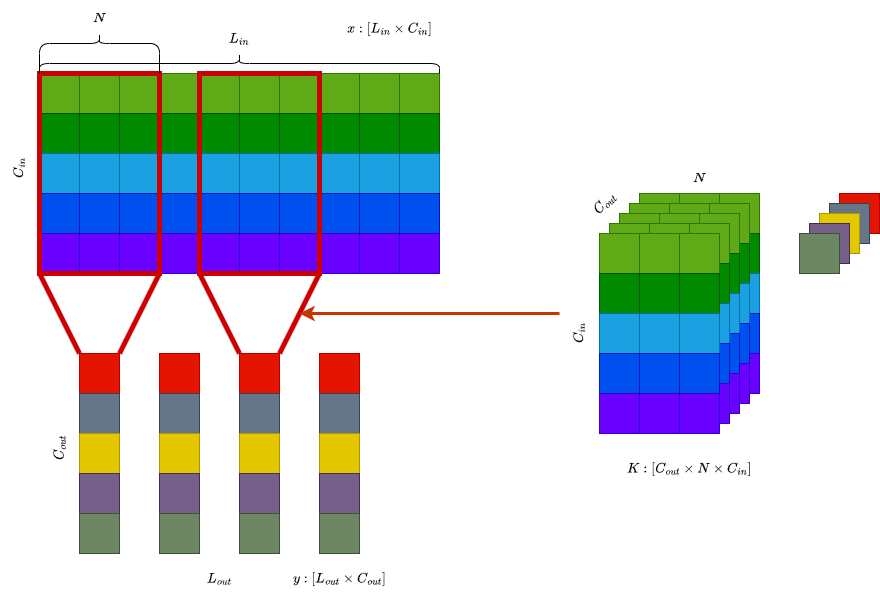
\includegraphics[width=0.9\linewidth]{figures/conv1d_drawio}
  \caption{Иллюстрации операции 1D свертки}
  \label{fig:conv1d_drawio}
\end{figure}

Каждый вектор $y_i: [1 \times C_{out}]$ можно рассматривать как матричное умножение вырезанного окна $x_i: [1 \times (N \cdot C_{in})]$ на матрицу $K^T: [(N \cdot C_{in}) \times C_{out}]$.

В случае, когда входным массивом является аудиосигнал, количество входных каналов $C_{in} = 1$, и можно несколько упростить формулу. 
\[x: [L_{in}], \quad K: [C_{out} \times N]\]
\begin{equation}
	y[i, c_{out}] = \sum_{j=0}^{N-1} x[i \cdot s + j] \cdot K[c_{out}, j]
\end{equation}


\textbf{Дискретное оконное преобразование Фурье (STFT)} можно посчитать через 1D свертку, если сформировать ядро $K_{\mathrm{stft}}: [N \times N]$ следующим образом:
\begin{equation}
	K_{\mathrm{stft}}[k, n] = e^{-i\pi \frac{(n - N/2) \cdot k}{N}} * w[n]
\end{equation}

\textbf{Дискретное вейвлет-преобразование (DWT)} можно построить с помощью свертки с таким ядром:
\begin{equation}
	K_{\mathrm{dwt}}[k, n] = \psi^* \left(\frac{n - N/2}{a_0^k}\right)
\end{equation}
\[\psi(t) = e^{i\pi t} * e^{-\left(\frac{\pi t}{2\sigma}\right)^2}, \quad   a_0 \in (1, \infty)\]

На рисунке \ref{fig:stft_kernel} изображены ядра сверток для указанных преобразований, а также для преобразования, которое будет описано в данной работе.

\begin{figure}
  \centering
  \subfigure{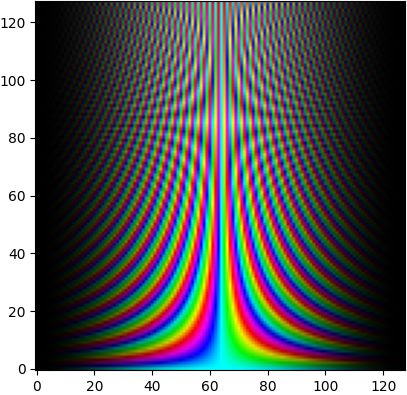
\includegraphics[width=0.3\textwidth]{figures/stft_kernel}} 
  \subfigure{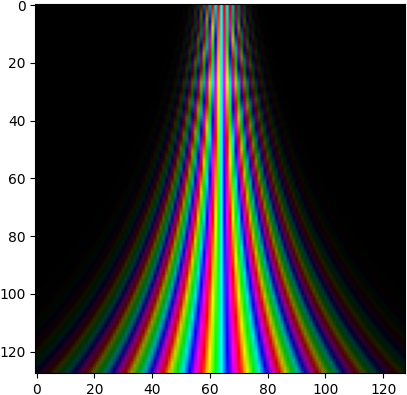
\includegraphics[width=0.3\textwidth]{figures/dwt_kernel}} 
  \subfigure{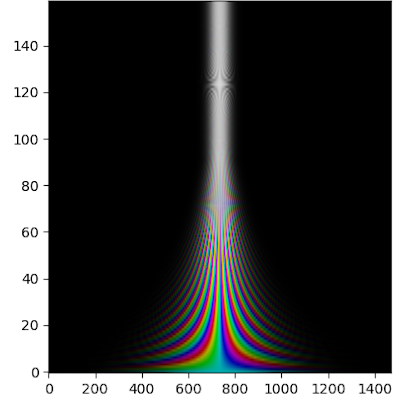
\includegraphics[width=0.3\textwidth]{figures/my_kernel}} 
  \caption{Ядро 1D свертки для STFT (1), вейвлет преобразования (2) и предлагаемого в работе преобразования (3)}
  \label{fig:stft_kernel}
\end{figure}





\begin{markdown}
 - Оконное фурье через свертку
   - метод, окна, частоты, неопределенность
   - вычислительная сложность
 - оптимальный размер окна для конкретной шкалы частот
 - оптимальная форма окна для устойчивости к искажениям
 - Восстановление сигнала через свертку
 - Критерий восстановимости
 - восстановление сигнала с наложением
 - шкала амплитуд
 - выбор оптимальной шкалы частот
   - мел шкала
   - линейная шкала
   - комбинированная шкала
 - рекомендуемые значения параметров
 - связь количества частот и разрешения по времени
 - точность восстановления
 - избыточность информации в шумах
 - представление с сохранением фазы
 - представление с производной фазы
 - представление с магнитудой
 - Алгоритм Гриффина-Лима
  - адаптация
  - более точное восстановление при сохранении фазы
 - картинки
\end{markdown}

\section{Реализация алгоритма}
\begin{markdown}
 - описание алгоритма
   - подготовка ядра
     - шкала частот, df
	 - окна для каждой частоты
	 - Фурье базис с окнами, нормировка
	 - маска наложений
	 - ядро прямого прохода
	 - ядро обратного прохода
   - прямое преобразование
     - свертка
	 - преобразование фазы
	   - либо ничего
	   - либо производная фазы
	   - либо только магнитуда
	 - шкала амплитуд
   - обратное преобразование
     - шкала амплитуд
	 - восстановление фазы
	   - либо ничего
	   - либо интеграл (при этом накапливаются ошибки)
	   - либо GriffinLim
	 - свертка
 - код на Python
 - предложения для быстрой реализации
 - ускорение на GPU и TPU
 - визуализация спектрограмм
\end{markdown}

\section{Выводы по главе}

\chapter{Полученные результаты}

В данной главе будут описаны эксперименты, проведенные для проверки качества и практической применимости алгоритма, и их результаты.
После чего будут даны рекомендации по применению алгоритма и планы его дальнейшего развития.

\section{Результаты экспериментов}
\label{sec:sec_3_1}

В разделе будет описаны проведенные для проверки качества алгоритма эксперименты.

\subsection{Прямой и обратный проход}
Самый простой эксперимент - построить спектрограмму из аудиосигнала, и сразу же преобразовать ее обратно в звук. 
После чего снова построить спектрограмму и сравнить спектрограммы исходного и восстановленного сигнала.

Эксперимент показал, что в случае с сохранением фазы, сигнал восстанавливается точно в области низких частот,
и в зависимости от выбора шага свертки, возможна погрешность в области высоких частот (см. Рисунок \ref{fig:spec_diff_results}).
Сравнение сгенерированных аудиозаписей показало, что человек не слышит этой разницы, что позволяет использовать 
больший шаг свертки, чем необходимый для точного восстановления.

\begin{figure}
  \centering
  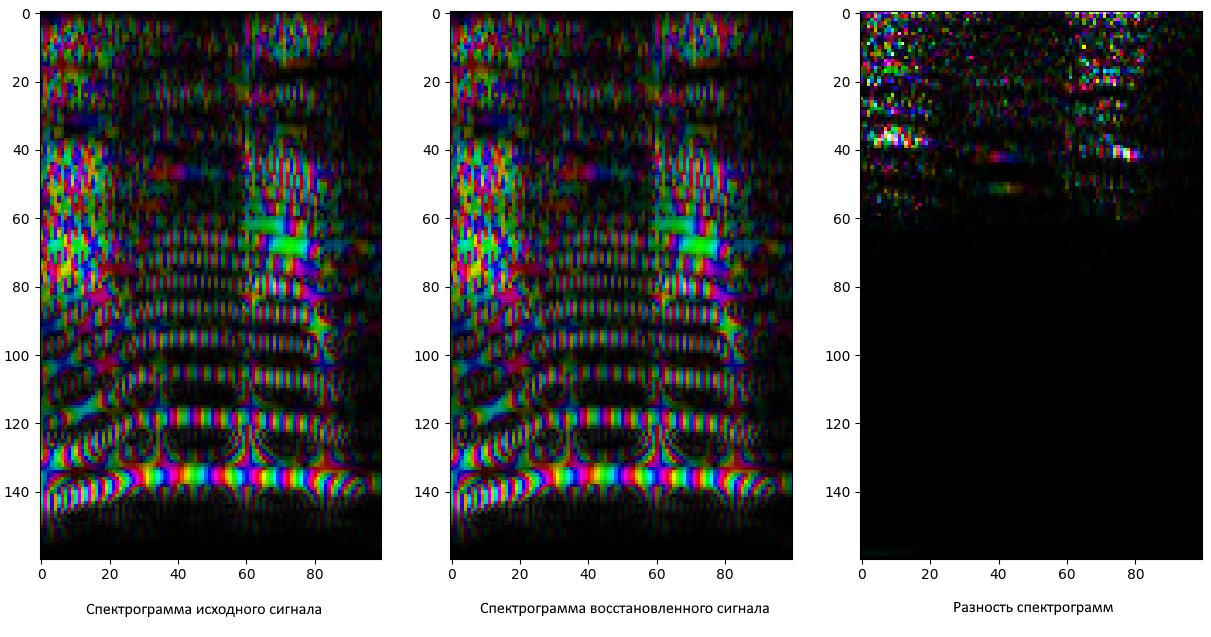
\includegraphics[width=0.8\linewidth]{figures/spec_diff}
  \caption{Спектрограмма сигнала до и после восстановления и их разность}
  \label{fig:spec_diff_results}
\end{figure}

В случае с восстановлением фазы с помощью алгоритма Гриффина-Лима расхождения с исходной спектрограммой присутствуют во всей частотной области
(см. Рисунок \ref{fig:spec_diff_griffinlim}). Но они тоже не слышны человеком, поскольку представляют собой незначительные сдвиги 
отдельных событий по времени в пределах нескольких шагов свертки.

\begin{figure}
  \centering
  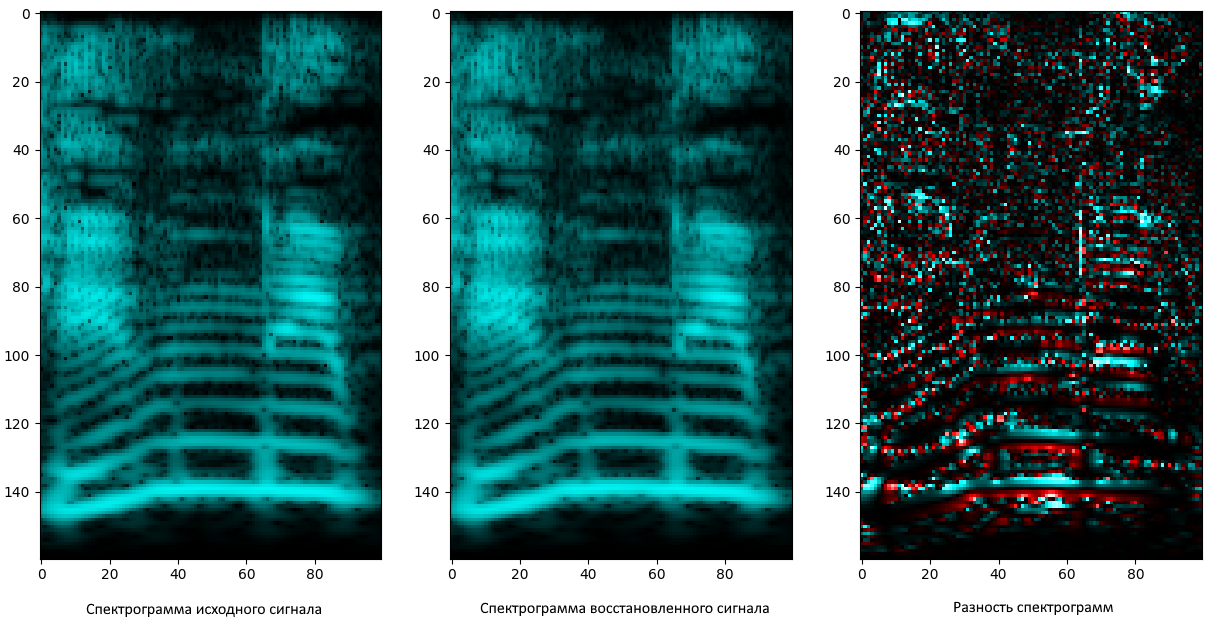
\includegraphics[width=0.8\linewidth]{figures/spec_diff_griffinlim}
  \caption{Спектрограмма сигнала до и после восстановления с реконструкцией фазы и их разность}
  \label{fig:spec_diff_griffinlim}
\end{figure}


\subsection{Устойчивость к трансформациям и искажениям}

Был произведен ряд экспериментов для определения устойчивости преобразования к трансформациям и искажениям. 

Исследовались следующие методы:
\begin{enumerate}[1.]
  \item Вейвлет-преобразование с сохранением фазы
  \item Вейвлет-преобразование с восстановлениме фазы с помощью адаптированного алгоритма Гриффина-Лима
  \item Классический алгоритм STFT и Гриффина-Лима в линейной шкале
\end{enumerate}

После построения спектрограммы она была подвергнута одному из следующих преобразований:
\begin{itemize}
  \item Добавление шума
  \item Сжатие и растяжение по времени
  \item Сжатие и растяжение по частоте
  \item Зануление случайных элементов
  \item Зануление прямоугольных участков
  \item Размытие участков
\end{itemize}

Из полученной спектрограммы восстанавливался аудиосигнал, качество которого сравнивалось с исходным на слух.
Результаты эксперимента приведены в таблице \ref{table:transform_exp}.
Если не было выявлено каких-либо артефактов, в ячейке ставится знак $+$.
Если выявлено незначительное ухудшение качества, ставится знак $\pm$.
Если качество значительно ухудшилось, ставится знак $-$.

\begin{table}[h!]
\centering

\begin{tabular}{||c c c c||} 
 \hline
  Трансформация \textbackslash \  Метод                & Сохр. фазы & Восст. фазы & GriffinLim \\ [0.5ex] 
 \hline\hline
  Добавление шума                      & $+$ & $+$ & $-$ \\
  Сжатие и растяжение по времени       & \pm & $+$ & \pm \\
  Сжатие и растяжение по частоте       & \pm & $+$ & \pm \\
  Зануление случайных элементов        & $+$ & $+$ & $-$ \\
  Зануление прямоугольных участков     & $+$ & $+$ & $-$ \\
  Размытие участков                    & \pm & \pm & $-$ \\ [1ex] 
 \hline
\end{tabular}
\caption{Устойчивость методов восстановления звука к трансформациям и искажениям}
\label{table:transform_exp}
\end{table}

В итоге, предлагаемый метод продемонстрировал ощутимое преимущество с точки зрения устойчивости к искажениям.


\subsection{Нейросетевой автоэнкодер представления с сохранененной фазой}
\label{subsec:keep_phase_net}

Для проверки гипотезы о возможности обучить нейросеть предсказывать сразу комплексное представление спектрограммы была обучена 
несложная нейронная сеть - автоэнкодер на основе архитектуры ResNet с 1D свертками. 
Пространственная размерность в конечном итоге сжималась в 8 раз.
Исходный шаг спектрограммы по времени соответствовал частоте 400 Гц.

В итоге эксперимента был получен следующий результат: Нейросеть смогла обучиться кодировать и декодировать когерентную часть спектрограммы
(гласные, звонкие согласные и т.д.) практически без потерь. Однако, шумоподобные данные (глухие согласные, шипящие) 
были утеряны, то есть, сглажены к нулевому среднему. 

Данный результат приводит к выводу, что подход с сохранением фазы возможен, но требуется отдельно обрабатывать шумоподобные данные: 
предсказывать не конкретную реализацию шума, а его стд. отклонение. Разделять спектрограмму на когерентный сигнал и шум можно как 
снаружи нейросети (как один из этапов преобразования), так и внутри сети 
(например предсказывать плавающее среднее и стд. отклонение, сравнивать их лосс-функцией с этими же параметрами эталона).


\subsection{Обучение Tacotron2 для работы с предлагаемым форматом}

В данном эксперименте была обучена модель синтеза речи Tacotron2 \cite{Tacotron2}. 
Был адаптирован готовый рецепт из open-source проекта Coqui-TTS \cite{coquiTTS}. 
В него была интегрирована реализация предлагаемого алгоритма для построения спектрограммы и восстановления звука.

В результате эксперимента получилась обученная модель, способная генерировать спектрограммы в предлагаемом вейвлет-представлении, 
которые потом декодировались в звук.

В качестве ближайших аналогов, с которыми производилось сравнение, были выбраны две следующие конфигурации:
\begin{itemize}
  \item Tacotron2 + HiFi-Gan - оригинал, обученные веса были заранее доступны в открытом доступе.
  \item Tacotron2 + GriffinLim - ближайший алгоритмический аналог. Ожидается, что по качеству будет заметно хуже первого варианта, и предлагаемый метод будет заметно лучше этого варианта.
\end{itemize}

Далее была произведена оценка качества звука. В качестве метрики для оценивания была выбрана метрика \textbf{Mean Opinion Score}, 
оцениваемая с помощью нейросети DNSMOS (Microsoft) \cite{dnsmos}. 
Выбор данной метрики обусловлен тем, что для ее расчета не требуется оригинал аудиозаписи для сравнения, поэтому ее можно использовать с 
генеративными моделями. Кроме того, она широко используется как одна из метрик качества в современных научных работах и признается научным сообществом.

Изначально, данная метрика оценивалась исходя из усредненной субъективной оценки группы пользователей, 
которым давали прослушать аудиозапись и предлагали выставить оценку качества от 1 до 5. 
Со временем накопилось достаточное количество данных, чтобы обучить нейросетевую модель, 
которая будет предсказывать данную оценку без необходимости собирать группу людей. Данный подход и был использован для оценки качества синтезируемого звука.
Результаты измерений представлены в таблице \ref{table:mos_tacotron}

\begin{table}[h!]
\centering

\begin{tabular}{||m{5cm} c c c||} 
 \hline
  Конфигурация \textbackslash \ Показатель &  Overall MOS & Signal MOS & Backgr. MOS \\ [0.5ex] 
 \hline\hline
  Tacotron2 + HiFi-Gan & 3.19 & 3.49 & 4.02 \\
  Tacotron2 + GriffinLim & 2.77 & 2.95 & 4.11 \\
  Tacotron2 (fine-tuned) + Новый декодер & \textbf{3.28} & \textbf{3.51} & \textbf{4.15} \\ [1ex] 
 \hline
\end{tabular}
\caption{Сравнение качества синтезированного звука по метрике MOS}
\label{table:mos_tacotron}
\end{table}

В результате проведенного эксперимента можно сделать вывод, что предлагаемый метод в сочетании с нейросетями 
позволяет достигать качества звука не хуже, чем нейросетевой декодер (напр. HiFi-Gan).


\section{Практическая ценность алгоритма}

Применение алгоритма в задачах синтеза речи позволит упростить архитектуру моделей за счет отсутствия необходимости в 
специализированном нейросетевом декодере. Также такой метод позволит улучшить переносимость и воспроизводимость моделей 
за счет использования стандартизируемого формата. 

Данный метод позвоялет декодировать звук без потери качества, что в перспективе может привести к достижению наилучших показателей 
качества синтезируемой речи. Также метод можно применить в задачах распознавания и анализа речи. 
Поскольку он позволяет получать более детальные спектрограммы, чем STFT, это может в теории улучшить точность распознавания речи.

Данный метод не требует существенных вычислительных затрат, что делает возможным его применение на мобильных и встраиваемых платформах
и повышает доступность технологий синтеза речи.

\section{Планы развития}

В процессе работы были выявлены точки развития алгоритма, позволяющие улучшить его показатели качества или быстродействия, 
либо уменьшить размеры спектрограммы при сохранении качества восстанавливаемого звука:

1. Разделение на когерентный сигнал и шум. В шуме хранится больше информации чем нужно, нужно сохранять только распределение, а не реализацию.

2. Голос и волны от резонаторов можно разложить на $f_0$ (pitch) и АЧХ резонатора. Если генерировать гармоники на основе $f_0$ 
и перемножать гармоники на АЧХ резонатора, можно будет легко менять pitch, сохраняя фонему. 
Это свойство можно использовать в музыкальных редакторах.

3. Реализация быстрого алгоритма для сервеных ускорителей, а также для мобильных и embedded платформ.

4. Разработка специализированной Text-to-Speech модели, использующей по максимуму все преимущества данного представления

\section{Выводы по главе 3}

Для оценки качества восстанавливаемого звука был проведен ряд экспериментов. 
Простые эксперименты показали, что предлагаемое преобразование устойчиво ко многим трансформациям и искажениям.

Также были проведены эксперименты для оценки качества работы алгоритма в сочетании с нейросетевыми моделями. 
Была успешно обучена модель Tacotron2 для работы с предлагаемым представлением спектрограммы.
В сочетании с разработанным алгоритмом декодирования звука обученная модель способна гененировать звук хорошего качества,
не хуже, чем оригинальная модель, использующая нейросетевой декодер.

Алгоритм имеет значимую практическую ценность благодаря тому, что позволит упростить архитектуру моделей, упростить и стабилизировать обучение,
сократить вычислительные затраты на обучение и исполнение моделей, в результате чего повысить доступность технологии для широкого круга пользователей.


\backmatter % Здесь заканчивается нумерованная часть документа и начинаются ссылки и заключение

\Conclusion % заключение к отчёту



\nocite{*}
\bibliographystyle{gost780u}
\bibliography{0-main}


\appendix   % Тут идут приложения

%\App
%\label{app}

\chapter{Приложение 1. Реализация алгоритма на языке Python}
\label{app:app1}

Реализация алгоритма выложена на платформу GitHub по адресу:
\url{https://github.com/LotusBro98/VoiceLab/blob/master/process.py}

Ниже представлен листинг реализации класса SpectrogramBuilder на языке Python. Этот класс реализует большинство описанных в работе функций.
Он использовался для проведения описанных в работе экспериментов.


\begin{verbatim}
import math
from typing import Literal, Optional
import matplotlib.pyplot as plt
import numpy as np
import torch
from torch import nn
from torch.nn import functional as F
from scipy.special import erfinv
from scipy.interpolate import interp1d


class SpectrogramBuilder(nn.Module):
    def __init__(self, 
                 sample_rate: float, 
                 fsave: float = 400,
                 n_feats: int = 160,
                 fmax: Optional[float] = None,
                 magnitude: bool = True,
                 hear_sense_threshold: float = 1e-0,
                 combo_scale: bool = True,
                 power_by_freq_scale: bool = True,         
        ):
        super().__init__()

        self.sample_rate = sample_rate
        self.fsave = fsave
        self.hear_sense_threshold = hear_sense_threshold
        self.n_feats = n_feats
        self.magnitude = magnitude
        self.combo_scale = combo_scale
        self.power_by_freq_scale = power_by_freq_scale

        self.fmin = 0
        self.fmax = fmax if fmax is not None else sample_rate / 2

        self.fn = self.get_mel_scale()
        self.build_kernel()

    def build_kernel(self):
        fn = self.get_mel_scale()
        df = torch.gradient(fn)[0]
        res = 2

        win_sizes = (self.sample_rate / df)[:, None]
        ksize = int(math.ceil(2 * torch.max(win_sizes)))
        self.stride = int(self.sample_rate / self.fsave)

        windows = self.get_window(ksize, win_sizes / res, ksize // 2)
        mask = self.get_window_mask(
            ksize, 
            self.stride, 
            windows.square()
        )

        t = (torch.arange(0, ksize) - ksize / 2) / self.sample_rate
        W = torch.exp(2j * torch.pi * fn[:, None] * t[None, :])
        W *= windows
        W /= win_sizes.sqrt()

        W_enc = W
        W_dec = W / mask * 2

        self.kernel_encode = torch.concat([
            W_enc.real,
            W_enc.imag
        ], dim=0)[:, None, :]

        self.kernel_decode = torch.concat([
            W_dec.real,
            W_dec.imag
        ], dim=0)[:, None, :]

    def _encode_conv(self, signal: torch.Tensor) -> torch.Tensor:
        if self.kernel_encode.device != signal.device:
            self.kernel_encode = self.kernel_encode.to(signal.device)
        sig_shape = signal.shape
        sig_len = signal.shape[-1]

        x = signal.reshape(-1, 1, sig_len)

        spec = F.conv1d(
            x, 
            weight=self.kernel_encode, 
            bias=None, 
            stride=self.stride,
            padding=0,
        )

        spec_real, spec_imag = spec.chunk(2, dim=1)
        spec = torch.complex(spec_real, spec_imag)

        spec = spec.reshape(sig_shape[:-1] + spec.shape[-2:])
        return spec
    
    def _decode_conv(self, spec: torch.Tensor) -> torch.Tensor:
        if self.kernel_decode.device != spec.device:
            self.kernel_decode = self.kernel_decode.to(spec.device)
        spec_shape = spec.shape

        spec = spec.reshape(-1, *spec_shape[-2:])

        spec = torch.concat([
            spec.real,
            spec.imag
        ], dim=1)

        signal = F.conv_transpose1d(
            spec, 
            weight=self.kernel_decode, 
            bias=None, 
            stride=self.stride,
            padding=0,
        )

        signal = signal.reshape(*spec_shape[:-2], signal.shape[-1])
        return signal
    
    def reconstruct_phase(self, spec_abs: torch.Tensor) -> torch.Tensor:
        # Griffin-Lim algorithm adaptation for signal reconstruction 
        # from magnitude-only spectrogram

        spec = torch.complex(spec_abs, torch.zeros_like(spec_abs))
        
        for i in range(100):
            signal = self._decode_conv(spec)
            spec = self._encode_conv(signal)
            spec = spec_abs * torch.exp(1j * spec.angle())

        return spec

    def encode(self, signal: torch.Tensor) -> torch.Tensor:
        spec = self._encode_conv(signal)
        if self.magnitude:
            spec = spec.abs()
        spec = self.to_bel_scale(spec)
        return spec
    
    def decode(
        self, 
        spec: torch.Tensor, 
        use_noise_masking: bool = True
    ) -> torch.Tensor:
        if use_noise_masking:
            f_thresh = 3000
            mask = F.sigmoid(
                (self.fn.to(spec.device) - f_thresh) / 
                self.n_feats
            )
            mask = mask[:, None] * torch.ones_like(spec)
            mask[spec < 1 * self.hear_sense_threshold] = 1

        if self.magnitude:
            spec = spec.clip(0, None)

        spec = self.from_bel_scale(spec)
        if self.magnitude:
            spec = self.reconstruct_phase(spec)
        
        if use_noise_masking:
            noise = torch.randn_like(spec) * spec.abs() * 1
            spec = spec * (1 - mask) + noise * mask

        spec[..., :1, :] = 0
        signal = self._decode_conv(spec)
        return signal
    
    def get_window(
        self, 
        n_save, 
        win_size, 
        shift=0, 
        kind: Literal[
            "flat", 
            "hann", 
            "gaussian", 
            "invflat", 
            "invhann"
        ] = "gaussian"
    ):
        window = (torch.arange(n_save) + shift + n_save // 2) % n_save - n_save // 2

        if kind == "hann":
            window = (
                torch.cos(
                    (window / win_size).clip(-1, 1) 
                    * torch.pi
                ) + 1) / 2
        elif kind == "flat":
            window = (window.abs() < win_size).float()
        elif kind == "invflat":
            win_size = n_save / win_size
            window = (window.abs() < win_size).float()
            window = torch.fft.ifft(window.roll(-shift))
                .clone().roll(shift)
        elif kind == "invhann":
            win_size = n_save / win_size
            window = (torch.cos((window / win_size).clip(-1, 1) * torch.pi) + 1) / 2
            window = torch.fft.ifft(window.roll(-shift)).clone().roll(shift)
        elif kind == "gaussian":
            prob_outside = 1e-2
            std = (win_size / 2) / erfinv(1 - prob_outside)
            window = torch.exp(-0.5 * torch.square(window / std))

        if kind not in ["invflat", "invhann"]:
            window -= window.abs().min()
        window /= window.max(-1, keepdim=True).values

        return window

    def get_window_mask(self, ksize, stride, windows):
        idxs = torch.concatenate([
            torch.arange(
                -ksize // stride * stride, 
                ksize // stride * stride, 
                stride
            )[1:-1]
        ])

        mask = torch.zeros_like(windows)

        for i in idxs:
            mask[:, max(i, 0): min(ksize + i, ksize)] += \
                windows[:, max(-i, 0): min(ksize - i, ksize)]

        return mask

    def freq_to_sample(self, freq):
        mel_min = self.freq_to_mel(self.fmin)
        mel_max = self.freq_to_mel(self.fmax)
        mel_x = self.freq_to_mel(freq)

        fn = (mel_x - mel_min) / (mel_max - mel_min) * self.n_feats
        return fn

    def sample_to_freq(self, fn):
        mel_min = self.freq_to_mel(self, self.fmin)
        mel_max = self.freq_to_mel(self, self.fmax)

        mel_x = fn / self.n_feats * (mel_max - mel_min) + mel_min
        freq = self.mel_to_freq(mel_x)

        return freq
    
    def _linear_tail_freq_scale(self, freqs):
        f_thresh = self.fsave / 4

        ii = torch.arange(1, self.n_feats)
        fs = freqs[1:]
        df = freqs[1:] - freqs[:-1]
        n_i = ii + (self.fmax - fs) / df
        scale = self.n_feats / n_i
        i_thresh = sum(df / scale < f_thresh)
        scale = scale[i_thresh]

        freqs = torch.concat([
            freqs[:i_thresh],
            torch.arange(freqs[i_thresh], self.fmax, f_thresh * scale)
        ])

        freqs = F.interpolate(
            freqs[None, None], 
            self.n_feats, 
            mode="linear"
        )[0, 0]

        return freqs

    def get_mel_scale(self):
        mel_min = self.freq_to_mel(self.fmin)
        mel_max = self.freq_to_mel(self.fmax)

        mels = torch.linspace(mel_min, mel_max, self.n_feats)
        freqs = self.mel_to_freq(mels)

        if self.combo_scale:
            freqs = self._linear_tail_freq_scale(freqs)

        return freqs

    def to_freq_diff_repr(
        self, 
        spectrum: torch.Tensor
    ) -> torch.Tensor:
        f = self.get_mel_scale() / self.fsave
        phase0 = torch.exp(2j * torch.pi * f[:, None])

        df = spectrum.angle()
        ampl = spectrum.abs()

        df = df.diff(1, -1, prepend=torch.zeros_like(df[..., :1]))

        df = (torch.exp(1j * df) * phase0).angle()

        spectrum = (
            ampl *
            torch.exp(1j * df)
        )

        return spectrum

    def from_freq_diff_repr(
        self, 
        spectrum: torch.Tensor
    ) -> torch.Tensor:
        f = self.get_mel_scale() / self.fsave
        phase0 = torch.exp(-2j * torch.pi * f[:, None])

        df = spectrum.angle()
        ampl = spectrum.abs()

        df = (torch.exp(1j * df) * phase0).angle()

        df = df.cumsum(-1)

        spectrum = (
            ampl *
            torch.exp(1j * df)
        )

        return spectrum

    def to_bel_scale(self, spectrum) -> torch.Tensor:
        ampl = spectrum.abs()
        if self.power_by_freq_scale:
            ampl = ampl * self.fn.to(ampl.device)[:, None]
        ampl = torch.log10(1 + ampl / self.hear_sense_threshold)

        if not torch.is_complex(spectrum):
            return ampl
        
        return (
            ampl *
            torch.exp(1j * spectrum.angle())
        )

    def from_bel_scale(self, spectrum) -> torch.Tensor:
        ampl = spectrum.abs()
        ampl = self.hear_sense_threshold * (torch.pow(10, ampl) - 1)
        if self.power_by_freq_scale:
            ampl = ampl / self.fn.to(ampl.device)[:, None]

        if not torch.is_complex(spectrum):
            return ampl

        return (
            ampl *
            torch.exp(1j * spectrum.angle())
        )
    
    def complex_picture(
        self, 
        spectrum: torch.Tensor, 
        ampl_cap: Literal["max", "std", None] = "std"
    ):
        ampl = spectrum.abs()
        if ampl_cap is None:
            pass
        elif ampl_cap == "std":
            ampl /= ampl.abs().square().mean().sqrt() * 3
        elif ampl_cap == "max":
            ampl /= ampl.max()

        phase = spectrum.angle()

        image = torch.stack([
            (phase + torch.pi).rad2deg(),
            (1 - ampl).clip(None, 0).exp(),
            ampl.clip(0, 1),
        ], dim=-1).float().numpy()

        import cv2 as cv
        image = cv.cvtColor(image, cv.COLOR_HSV2RGB)

        return image

    def mel_to_freq(self, mel):
        if not isinstance(mel, torch.Tensor):
            mel = torch.tensor(mel)
        return 700 * (torch.exp(mel / 1127) - 1)

    def freq_to_mel(self, freq):
        if not isinstance(freq, torch.Tensor):
            freq = torch.tensor(freq)
        return 1127 * torch.log(1 + freq / 700)

\end{verbatim}



\end{document}
